%&latex
% UF Sample ETD Main Document Fall 2016
% Documenting the conversion to xelatex compilation method
% Improved method of handling the single/multiple appendices issue
% Updated font calls to meet latest LaTeX standards

\documentclass[12pt,final,CPage]{ufthesis} %Use this line for Windows OS

% For those still using pdflatex and similar compilation methods - If you get a dvipdfm file not found error
% remove the dvipdfm and/or dvipdfmx options here and in the packages.tex file graphicx and hyperref packages and
% compile using Latex, Latex, Bibtex, Latex, Latex, XeLaTeX - this usually fixes
% the problem 

%-------------------------------------C:\Program Files\MiKTeX 2.5\miktex----------------------------------%
% Preamble %

% Define Packages To be used and options NOTE: If you add any packages please add them before the hyperref package%
% here you define all the packages you wish to use in your paper, the ones shown are not all necessary,
% but all have purpose and can be very useful, so leave these as default and add packages as necassary
%\usepackage{graphicx}
%\usepackage[dvipdfmx]{graphicx}
\usepackage{amsmath}
\usepackage{mathtools}
\usepackage{amsthm}
\usepackage{algpseudocode}
%\usepackage{algorithm}
\usepackage{tabularx}
\usepackage{url}
%\usepackage[letterpaper,hmargin=1in,vmargin=1in]{geometry}
\usepackage{pdflscape}
%\usepackage{hanging}
\usepackage{longtable}
\usepackage{amsfonts}
\usepackage{amssymb}
%\usepackage[cmss]{sfmath} % Comment this line to use Times New Roman Math Typeface
\usepackage[cmbright]{sfmath} % Comment this line to use Times New Roman Math Typeface
\usepackage{subfigure}
%\usepackage{subfig}
\usepackage{rotating}
\usepackage{calc}
\usepackage{setspace}
\usepackage{ufenumerate}
\usepackage{latexsym}
%\usepackage{epsf}
\usepackage{epsfig}
\usepackage{euscript}
\usepackage{multirow}
\usepackage[section]{placeins}
%\usepackage[subsection]{placeins}
\usepackage[format=hang,justification=raggedright,singlelinecheck=0,labelsep=period]{caption}
%\usepackage{cite}
\usepackage[numbers,sort&compress]{natbib} %Use this set-up for numbered reference lists
%\usepackage[authoryear]{natbib} %Use this set-up if you want an un-numbered reference list
%\usepackage{hypernat}



\usepackage[hyperfootnotes=false]{hyperref}
%\usepackage[dvipdfmx,hyperfootnotes=false]{hyperref}
%\usepackage[dvips,hyperfootnotes=false]{hyperref}
\hypersetup{colorlinks=true,linkcolor=blue,anchorcolor=blue,citecolor=blue,filecolor=blue,urlcolor=blue,bookmarksnumbered=true,pdfview=FitB} %
% % %DO NOT PLACE ANY PACKAGES AFTER THE HYPERREF SET UP


\usepackage{braket}
%\def\UrlFont{\rmfamily} %use this line for Times New Roman
\def\UrlFont{\sffamily} %use this line for CMSS

%\allowdisplaybreaks  % % This command allows equation arrays and similar environments
% % % to break across pages to improve text flow - use only if needed.

% Prevent figures, tables or algorithms from using a separate page or column alone
\renewcommand{\topfraction}{0.85}
\renewcommand{\textfraction}{0.1}
\renewcommand{\floatpagefraction}{0.75}

% *** Do not adjust lengths that control margins, column widths, etc. ***
% *** Do not use packages that alter fonts (such as pslatex).         ***
% There should be no need to do such things with IEEEtran.cls V1.6 and later.
% correct bad hyphenation here
%\hyphenation{op-tical net-works semi-C:\Program Files\MiKTeX 2.5\miktexconduc-tor}

%------------------------------------------%

% Extra commands or misc formatting such as page alignment or output paper-size commands

%\include{extraparameters}

%------------------------------------------%

% Set your personal and paper information
\SetFullName{Andrew Carnes}%
\SetThesisType{Dissertation}%{Dissertation} %{Thesis}
\SetDegreeType{Doctor of Philosophy}% {Doctor of Philosophy} {Master of Science}
\SetGradMonth{December}%
\SetGradYear{2017}%
\SetDepartment{Physics}%
\SetChair{Paul Avery}%
%\SetCochair{John W. Carver III}%uncomment this line and enter the name of your cochair inside the braces if you have one.
%If you have a cochair there two places in the ufthesis.cls file that will need to be uncommented as well
%In the "getting personal information" section about line 630
%And the "Abstract" Section around line 556
% Type your title here in all CAPS %
\SetTitle{A SEARCH FOR THE STANDARD MODEL HIGGS DECAYING TO TWO MUONS AT THE CMS EXPERIMENT}


%------------------------------------------%

% user defined commands in order to geC:\Program Files\MiKTeX 2.5\miktexnerate new commands, macros, and redefine default commands %
% user defined commands %
% Here is where you define optional commands such as macros, new commands,
% and new environments to be used in your paper

% optional command to prevent a word from breaking across a line %
\hyphenchar\font=-1


% Commands to produce proper bullet list
\newlength{\widthOfItem}
\let\Itemize=\itemize
\let\endItemize=\enditemize
\renewenvironment{itemize}{%
	\begin{Itemize}
		\setlength{\itemsep}{0.5\baselineskip}
		\setlength{\labelwidth}{2em}
		\setlength{\listparindent}{.32in}%
		\setlength{\leftmargin}{.32in}
		\setlength{\rightmargin}{0in}
		\settowidth{\widthOfItem}{\labelitemi}
		\setlength{\labelsep}{\leftmargin-\widthOfItem}
		\renewcommand{\labelitemii}{--}
		\singlespacing}{%
	\end{Itemize}}

% shortcut for setting up inserting \prime command in mathmode to avoid errors %
\newcommand{\p}{^{\prime}}

% shortcuts for prime color text
\newcommand{\red}{\textcolor[rgb]{1.00,0.00,0.00}}
\newcommand{\green}{\textcolor[rgb]{0.00,1.00,0.00}}
\newcommand{\blue}{\textcolor[rgb]{0.00,0.00,1.00}}

% Shorcut commands for mathmatical formulas %

\newcommand{\latex}{\LaTeX 2\ensuremath{\epsilon}}

% THEOREM Environments ---------------------------------------------------
%These environments are provided as a convenience - feel free to modify if needed

\newtheorem{theorem}{Theorem}[chapter]%To link the theorem to each chapter uncomment the chapter option
\newtheorem{lemma}{Lemma}%[theorem]% To link each lemma to a theorem uncomment the theorem option
\newtheorem{corollary}{Corollary}%[theorem]% To link each corollary to a theorem uncomment the theorem option
% to link a corollary to a chapter change the theorem option to chapter
\newtheorem{definition}{Definition}%[chapter] %the same is true for both definitions and assumptions
\newtheorem{assumption}{Assumption}%[chapter] %
\newtheorem{proposition}{Proposition}[chapter]
\newtheorem{algorithm}{Algorithm}[chapter]


%These were some user commands I've run across that I thought some might want to incorporate into their work
%\newcommand{\bdm}{
 %   \begin{displaymath}}

%\newcommand{\edm}{
%    \end{displaymath}}

%\newcommand{\be}{
%    \begin{equation}}

%\newcommand{\ee}{
%    \end{equation}}

%\newcommand{\bea}{
 %   \begin{eqnarray}}

%\newcommand{\eea}{
%    \end{eqnarray}}


%-------------------------------------------------------------------------------------------------------%

% Begin Main Part of Document %

\begin{document}


 % % % % % % % % % % % % % % % % % % % % % % % % % % % % % % % % % % % % % %
 % Remember - You MUST get a .bst file that matches the Journal in your
 % field that you choose as your Reference example
 % NONE of these examples will satisfy the Graduate Editorial Office
 % if they don't match your Journal example!!!!
 % NOTE: If you use a numbered reference system and your references
 % are set in parentheses rather than brackets you need to select the
 % Natbib option "numbers sort and compress" in the packages.tex file
 % % % % % % % % % % % % % % % % % % % % % % % % % % % % % % % % % % % % % %


 %Note that the path separator is a forward slash NOT a back slash
 %Place YOUR .bst file in the bst folder and use that filename (without the .bst extension)
 % as your Bibliography Style file

%\bibliographystyle{bst/abbrv}
%\bibliographystyle{bst/abbrvnat}
%\bibliographystyle{bst/abbrvurl_uf}
%\bibliographystyle{bst/alphaurl_uf}
%\bibliographystyle{bst/apa-good}
%\bibliographystyle{bst/Chicago_Web}
%\bibliographystyle{bst/ecology_web}
%\bibliographystyle{bst/IEEEtran}
%\bibliographystyle{bst/mla_web}
\bibliographystyle{bst/mla-good}
%\bibliographystyle{bst/plainnat}
%\bibliographystyle{bst/plainurl_uf}
%\bibliographystyle{bst/Science_Web}
%\bibliographystyle{bst/uf_econ}
%\bibliographystyle{bst/uffull}
%\bibliographystyle{bst/ufinit}
%\bibliographystyle{bst/unsrtnat}
%\bibliographystyle{bst/unsrturl_uf}
%\bibliographystyle{bst/plain}
%\bibliographystyle{bst/ufinit}
%\bibliographystyle{bst/plainurl_uf}


%-----------------------------------------------------------------------%

\maketitle % % % % Creates the Title page from the information entered in userinfo.tex
\makecopyright

%------------------------------------------%

%\dedication{% Add your text for the dedication here between the center tags
%\addvspace{4.25in}
%\begin{center}%\singlespacing
\vspace{-20 mm}
I dedicate this to everyone that helped revamp this template. Aliquam molestie sed urna quis convallis. Aenean nibh eros, aliquam non eros in, tempus lacinia justo. In magna sapien, blandit a faucibus ac, scelerisque nec purus. Praesent fermentum felis nec massa interdum, vel dapibus mi luctus. Cras id fringilla mauris. Ut molestie eros mi, ut hendrerit nulla tempor et. Pellentesque tortor quam, mattis a scelerisque nec, euismod et odio. Mauris rhoncus metus sit amet risus mattis, eu mattis sem interdum.\\
%\end{center}
} % %Creates the dedication - if your dedication is more than a single line
% % % % % % % % % % % % % % % % % %you will need to reduce the vspace amount to keep the text centered verticlly
% % % % % % % % % % % % % % % % % %optional - comment or delete if you are not dedicating to anyone,

%------------------------------------------%

% Make sure to keep the text within the brackets and the output should turn out correct
\acknowledge{%
I would like to thank my Mom and Dad for all of their support throughout my life, making the completion of this Ph.D possible. I would also like to thank Professors Paul Avery and Darin Acosta for their support. Moreover, I would like to thank Andrew Brinkerhoff and Pierluigi Bortignon for all of their help in answering my many questions.}
 % % % %Required - There is no requirement to acknowledge a particular person
% % % % % % % % % % % % % % % % %but you must acknowledge someone (funding source, committee chair, spouse)?

%------------------------------------------%

% This file includes the file which creates the table of contents %
% This creates your table of contents, list of figures, and list of tables
% the pdfbookmark line adds the word to the bookmarks of the pdf without adding it to the TOC itself
\pdfbookmark[0]{TABLE OF CONTENTS}{tableofcontents}
\tableofcontents %
\listoftables %
%\setcounter{lofdepth}{2}
\listoffigures %

% Produced list of abbreviations or symbols %
%\printindex[keylist]{KEY TO ABBREVIATIONS}{KEY TO ABBREVIATIONS}{}
%\printindex[mathlist]{KEY TO SYMBOLS}{KEY TO SYMBOLS}{%
%The list shown below gives a brief description of the major mathematical symbols defined in this work. For each
%symbol, the page number corresponds to the place where the symbol is first used.} %
 %This file creates the Table of Contents, List of Figures, and List of Objects (if any)
% % % % % % % %delete or comment the file you want to remove

%------------------------------------------%

%%This is an optional file. A list of abbreviations is NOT even suggested.
%%Best practice is to define the item the first time it is used in the document

%%%-----------List of Symbols, Nomenclature or Abbreviation--------

%% Please note: a list of Symbols, terms, acronyms, etc. is not usually the best practice.
%% More often you should simply define an abbreviation the first time it is used.
%% If you DO need to include a list like this please notice that it must be paginated manually
%% by breaking it up into page size tables. Longtable will not wrap the definition properly if
%% it extends to a second line and a similar issue is encountered when the tabbing environment
%% is used. If you have a better way of meeting the Editorial Office requirements I'd love to hear about it.

\chapter*{LIST OF SYMBOLS, NOMENCLATURE, OR ABBREVIATIONS} \addcontentsline{toc}{chapter}{LIST OF SYMBOLS} %Start
%writing here. This is optional.
\singlespacing
\begin{tabular}{l p{5in}} %if the terms in the first column are longer than 1.4 inches reduce the number 5 appropriately
$\sum$ & Denotes the summation of a series of terms\\
\\%This adds the single space between definitions (required)
$\bigcap$ & A really big bigcap\\
\\
fractal & A geometric pattern that is repeated at ever smaller
scales to produce irregular shapes and surfaces that cannot be represented by classical
geometry. Fractals are used especially in computer modeling of irregular patterns and structures in nature.}\\
\\
polynomial & (in one variable) an expression consisting of the sum of two
or more terms each of which is the product of a constant and a
variable raised to an integral power: $ax^2 + bx + c$ is a
polynomial, where $a, b,$ and $c$ are constants and $x$ is a
variable.}\\
\\
$\sum$ & Denotes the summation of a series of terms\\
\\
$\bigcap$ & A really big bigcap\\
\\
fractal & A geometric pattern that is repeated at ever smaller
scales to produce irregular shapes and surfaces that cannot be represented by classical
geometry. Fractals are used especially in computer modeling of irregular patterns and structures in nature.}\\
\\
polynomial & (in one variable) an expression consisting of the sum of two
or more terms each of which is the product of a constant and a
variable raised to an integral power: $ax^2 + bx + c$ is a
polynomial, where $a, b,$ and $c$ are constants and $x$ is a
variable.}\\
\\
$\sum$ & Denotes the summation of a series of terms\\
\\
$\bigcap$ & A really big bigcap\\
\\
fractal & A geometric pattern that is repeated at ever smaller
scales to produce irregular shapes and surfaces that cannot be represented by classical
geometry. Fractals are used especially in computer modeling of irregular patterns and structures in nature.}\\
\\
polynomial & (in one variable) an expression consisting of the sum of two
or more terms each of which is the product of a constant and a
variable raised to an integral power: $ax^2 + bx + c$ is a
polynomial, where $a, b,$ and $c$ are constants and $x$ is a
variable.}\\

\end{tabular}

\begin{tabular}{lp{5in}}
$\sum$ & Denotes the summation of a series of terms\\
\\
$\bigcap$ & A really big bigcap\\
\\
fractal & A geometric pattern that is repeated at ever smaller
scales to produce irregular shapes and surfaces that cannot be represented by classical
geometry. Fractals are used especially in computer modeling of irregular patterns and structures in nature.}\\
\\
polynomial & (in one variable) an expression consisting of the sum of two
or more terms each of which is the product of a constant and a
variable raised to an integral power: $ax^2 + bx + c$ is a
polynomial, where $a, b,$ and $c$ are constants and $x$ is a
variable.}\\
\\
$\sum$ & Denotes the summation of a series of terms\\
\\
$\bigcap$ & A really big bigcap\\
\\
fractal & A geometric pattern that is repeated at ever smaller
scales to produce irregular shapes and surfaces that cannot be represented by classical
geometry. Fractals are used especially in computer modeling of irregular patterns and structures in nature.}\\
\\
polynomial & (in one variable) an expression consisting of the sum of two
or more terms each of which is the product of a constant and a
variable raised to an integral power: $ax^2 + bx + c$ is a
polynomial, where $a, b,$ and $c$ are constants and $x$ is a
variable.}\\
\\
$\sum$ & Denotes the summation of a series of terms\\
\\
$\bigcap$ & A really big bigcap\\
\\
fractal & A geometric pattern that is repeated at ever smaller
scales to produce irregular shapes and surfaces that cannot be represented by classical
geometry. Fractals are used especially in computer modeling of irregular patterns and structures in nature.}\\
\\
polynomial & (in one variable) an expression consisting of the sum of two
or more terms each of which is the product of a constant and a
variable raised to an integral power: $ax^2 + bx + c$ is a
polynomial, where $a, b,$ and $c$ are constants and $x$ is a
variable.}\\
\\
\end{tabular}
\doublespacing




%------------------------------------------%
% This line adds the word CHAPTER to the TOC just before the listing of the chapter and subsections begins
\addtocontents{toc}{\protect\addvspace{10pt}\noindent{CHAPTER}\protect\hfill\par}{}% This extra line adds the word CHAPTER to the table of contents %
\phantomsection
% Write in only the text of your abstract, all the extra heading jargon is automatically taken care of
\begin{abstract}
In 2012 two collaborations at the Large Hadron Collider announced the discovery of a new particle with properties similar to the Standard Model Higgs Boson. In order to determine whether the boson discovered with a mass of 125 GeV is actually the Standard Model Higgs, all of the different ways the particle can decay need to be investigated. If the probabilities for the different decays do not match the predictions of the Standard Model then this would imply new physics. 

This dissertation presents the search for the Standard Model Higgs Boson decaying to $\mu^{+}\mu^{-}$. The search uses the $35.9\pm0.9$~fb$^{-1}$ of $\sqrt{s}$ = 13 TeV proton-proton collision data recorded by the CMS detector in 2016. The signal strength ($\mu = (\sigma\mathcal{B})/(\sigma\mathcal{B})_{SM}$) is measured at $0.7^{+1.1}_{-1.0}$ for $m_H=125$ GeV, where $\sigma$ is the Higgs production cross section and $\mathcal{B}$ is the branching fraction to muons. The observed and expected upper limits on the signal strength at a 95 \% confidence level are presented for Higgs masses in the range 120 to 130 GeV. The observed and expected upper limits at a mass of 125 GeV are 2.64 and 2.08 $\times$ respectively. The significance is reported in the same range, and the observed and expected significance at $m_H=125$ GeV are 0.98$\sigma$ and 0.74$\sigma$ respectively. 

Combined results for 5.0 $fb^{-1}$ of 7 TeV, 19.8 $fb^{-1}$ of 8 TeV, and 35.9 $fb^{-1}$ of 13 TeV data are also presented. For $m_H=125$ GeV, the combination yields a measured signal strength of $0.9^{1.0}_{-0.9}$, observed (expected) upper limits at 95\% confidence of 2.64 (1.89), and an observed (expected) significance of 0.98 (1.09)$\sigma$. The results correspond to an upper limit on the $H\rightarrow\mu^+\mu^-$ branching fraction of 5.7x10$^{-4}$. These results provide the best results to date on the Higgs coupling to second generation fermions. No deviations from the Standard Model are observed. 
\end{abstract}
 %The abstract is created using this file and userinfo.tex
% % % % % % % % % % %If you have a c-chair you must uncomment that line in userinfo.tex AND find the
% % % % % % % % % % %co-chair lines in ufthesis.cls and un-comment those as well

%-----------------------------------------------------------------------%

% This section encompasses the main body of the paper from all the content through to the biographical sketch

% Chapters to be included (more can be added by creating a new chapter#.tex %
% file and then implementing the \inlcude{chapter#.tex} command as seen below %
\chapter{INTRODUCTION} \label{intro}

The Standard Model (SM) of particle physics is an extremely successful theory shown to correctly predict the behavior of the particles and forces which make up the most basic constituents of the universe. In fact, it correctly describes all of the forces known except for gravity \cite{smnograv}. In particular, the SM predicts that the massive particles of the theory acquire their mass by interacting with a scalar particle called the Higgs boson \cite{higgs1,higgs2,higgs3,qftam}. On July 4, 2012 two collaborations at the Large Hadron Collider (LHC), the A Toroidal LHC Apparatus (ATLAS) and Compact Muon Solenoid (CMS), announced the discovery of a new boson at 125 GeV with properties similar to the Standard Model Higgs \cite{atlasdiscovery,cmsdiscovery2012,cmsdiscovery2013}. This discovery was fueled by the investigation into the Higgs decays to the vector bosons ZZ and ${\rm \gamma\gamma}$. Soon after, evidence for the Higgs coupling to matter was found through the ${\rm \tau^{+}\tau{-}}$ and ${\rm b\bar{b}}$ decays \cite{cmshiggstau,cmshiggsbb,cmshiggsferm,atlashiggsbb}. Whether the newly discovered boson is indeed the expected Standard Model Higgs remains to be determined. Insofar, all of the different decay modes will be investigated to search for deviations from the Standard Model predictions.

This leads to the study of the Higgs decay to $\mu^{+}\mu^{-}$. Although this decay is the smallest branching fraction expected to be detected \cite{smallestbranch1,smallestbranch2}, the dimuon decay offers high efficiency and excellent momentum resolution, which should lead to a narrow peak over the falling background, mostly Drell Yan events. The tiny branching fraction enables greater sensitivity to small deviations from the predicted decay rate and in this respect offers an advantage over other channels where a miniscule deviation could be drowned out. Furthermore, the Higgs coupling to second generation fermions remains to be determined. 

This dissertation presents the search for the Standard Model Higgs Boson decaying to $\mu^{+}\mu^{-}$ using the proton-proton collision data recorded by the CMS experiment in 2016. In order to maximize the data available for the search, the first machine learning in the L1 Trigger system at the LHC is developed and deployed for 2016 data collection. To further maximize the sensitivity of the search, an additional machine learning technique is invented to categorize events based upon the detector resolution and the event kinematics. The search looks for a Higgs boson with a mass between 120 and 130 GeV and presents the expected and observed upper limits on the rate of $H\rightarrow\mu^+\mu^-$ production in this range as well as the p-values on the background-only hypothesis. The best fit for the rate of production is also presented. The 13 TeV results are then combined with the 2012 $H\rightarrow\mu^+\mu^-$ results on 7 and 8 TeV data \cite{cmshiggsmumu2012}.  

The dissertation first covers the LHC which accelerates and collides the protons. The dissertation then presents the CMS detector which measures the paths, momentum, and energy of the emerging particles. Next, the dissertation explains the theory underlying the Standard Model and its predictions of the Higgs particle. After, the machine learning implementation in the L1 trigger that reduced the number of fakes in the data by a factor of three is detailed. Finally, the search for H to $\mu^{+}\mu^{-}$ is presented.

\chapter{THE LARGE HADRON COLLIDER AND THE CMS EXPERIMENT} \label{lhc-cms}

\section{Large Hadron Collider}
The Large Hadron Collider is a particle collider near Geneva, Switzerland run by the European Organization for Nuclear Research (CERN). The LHC is the largest and most powerful particle collider ever built, designed to collide protons with a center of mass energy of 14 TeV and a luminosity of $10^{34} {\rm cm^{-2}s^{-1}}$ \cite{LHC}. The luminosity is given by

\begin{equation}
L = \frac{n_{b} f N^{2}_{p} \gamma}{4\pi\epsilon_{n}\beta^{*}}
\end{equation}
where $n_{b}$ is the number of bunches in each ring, f is the frequency for a bunch to circle the ring, ${\rm N_{p}}$ gives the number of protons in a bunch, and ${\rm \gamma}$ is the Lorentz factor. ${\rm \epsilon_{n}}$ is the normalized transverse emittance, a measure of the spread of the beam in momentum and position space. ${\rm \beta^{*}}$ measures the focus of the beam at the interaction point. ${\rm \epsilon_{n}\beta^{*}}$ represents the transverse area at the point of interaction. A large luminosity is characterized by a high frequency of bunch crossings with lots of protons in each bunch packed as densely as possible, and a large luminosity results in a high rate of collisions. With many collisions at high energy, the detectors can collect enough events from yet unexplored regimes of physics to discover new physics or to verify or discard the predictions different hypothesis, so these parameters are very important. 

The collider itself is 26.7 km in circumference 45-170 m underground. 8.3 T supercooled superconducting magnets operating at 2 K steer the high energy proton beams. In order to save money the LHC not only reuses the tunnels of a previous collider, the Large Electron Positron Collider (LEP), but also reuses older accelerators which were state of the art at their time. These older accelerators ramp up the energy of the protons and inject them into the LHC. All of this together makes up the CERN accelerator complex.

\begin{figure}[h!]
  \centering
  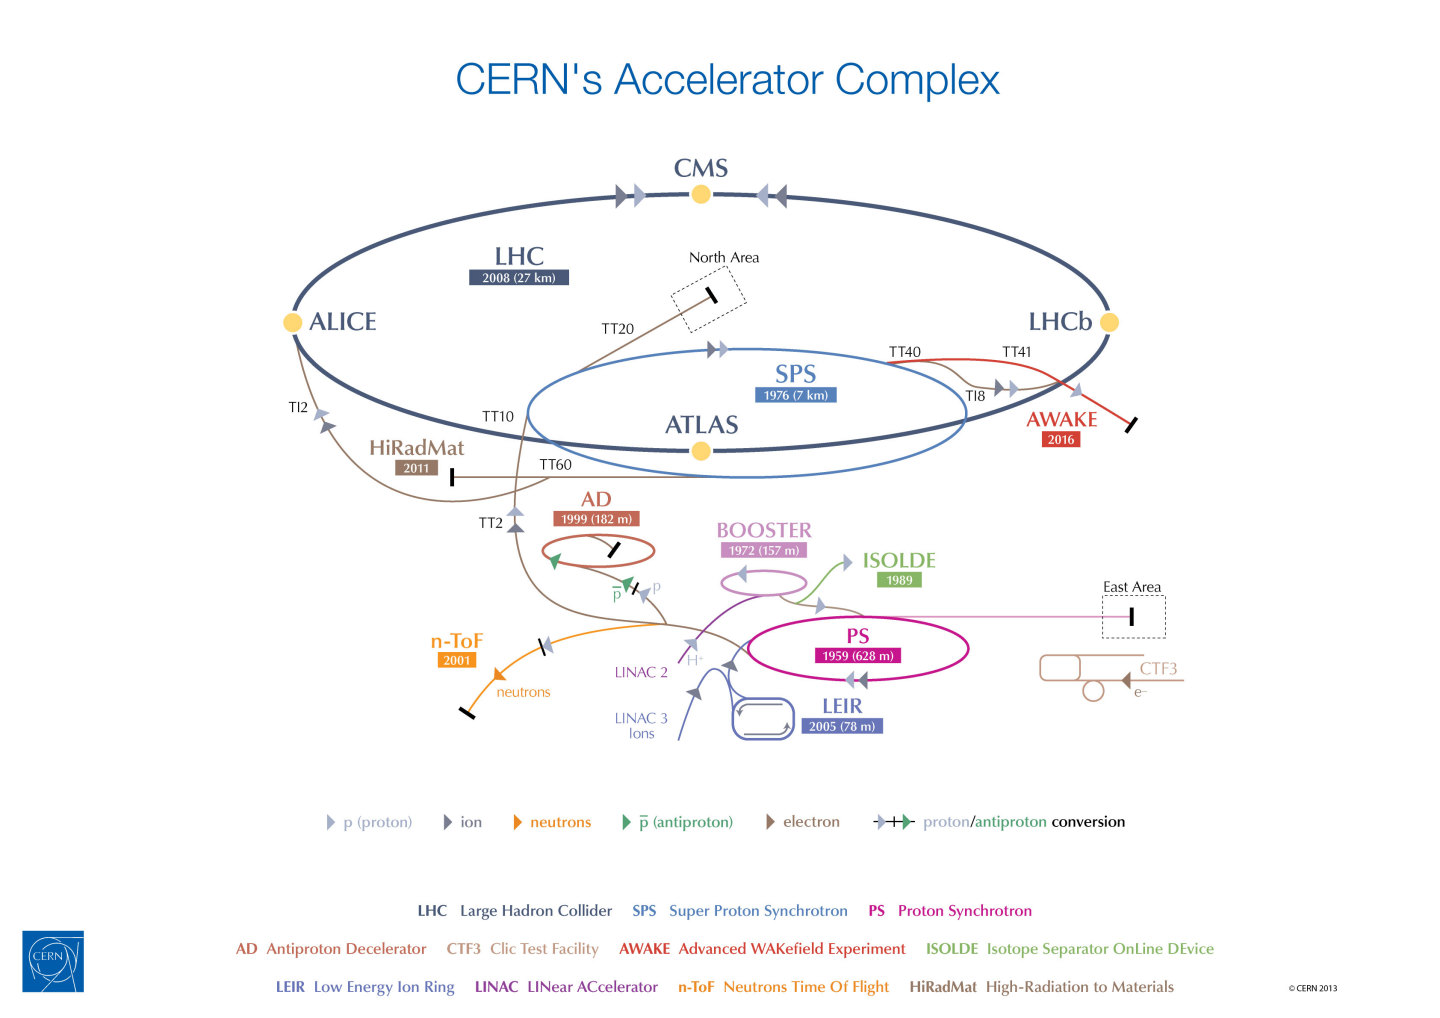
\includegraphics[width=6in]{images/cern_accel_complex.png}
  \caption
   {The CERN Accelerator Complex \cite{cernaccelcomplex}}
  \label{fig:cernaccel}
\end{figure}

First, the protons are created from a source of Hydrogen gas. The hydrogen atoms of the gas are placed into a large electric field that separates the atoms into unbound protons and electrons. The protons are then sent to a radio frequency quadrapole which focuses the protons and accelerates them. The radio frequency field is stronger for the protons in the back than in the front and consequently squeezes them into a tighter bunch. The protons then proceed to a linear accelerator, LINAC2, where they are accelerated to 50 MeV or 5\% of the speed of light (c). The protons then enter a series of synchrotrons. A synchrotron is a device that accelerates particles by guiding them around a fixed circular path with a magnetic field and boosting their speed with an electric field as they pass a certain point. Since a faster particle bends less in the same magnetic field, the magnetic field strength is synchronized with the speed of the accelerating particles to keep them in the fixed circular path. 

After LINAC2 the protons enter the first of the synchrotrons, the Proton Synchrotron Booster (PSB) accelerating the protons to 1.4 GeV (0.81c). From here the protons are injected into the Proton Synchrotron (PS) and accelerate to 25 GeV (0.999c). The PS then injects the protons into the Super Proton Synchrotron (SPS) further accelerating them to 450 GeV (0.99999c). Finally the protons are injected into the LHC where they accelerate up to 6.5 TeV (0.99999999c). Once accelerated to the appropriate collision energy, the proton beams are made to collide in the different detectors located around the ring. By colliding enough protons at large enough energies it is possible to probe corners of physics that have never been seen before. The two general purpose detectors at the LHC, ALTAS and CMS, are used to look for signs of new physics like the Higgs boson, dark matter, and extra dimensions by measuring the energy, the momentum, and the paths of the particles coming out of the collisions.

\section{Compact Muon Solenoid Detector}

The CMS detector, located in Cessy, France, is 21.6 m long, 15 m in diamater, and weighs more than the Eiffel Tower. Not only is the detector a massive and complex device it's also run by a huge collaboration involving approximately 3,800 people from 200 institutes spanning 43 different countries \cite{cmscollab}. The greatest achievement of the collaboration to date is the discovery of a Higgs like particle in 2012, a feat shared with ATLAS.

\begin{figure}[h!]
  \centering
  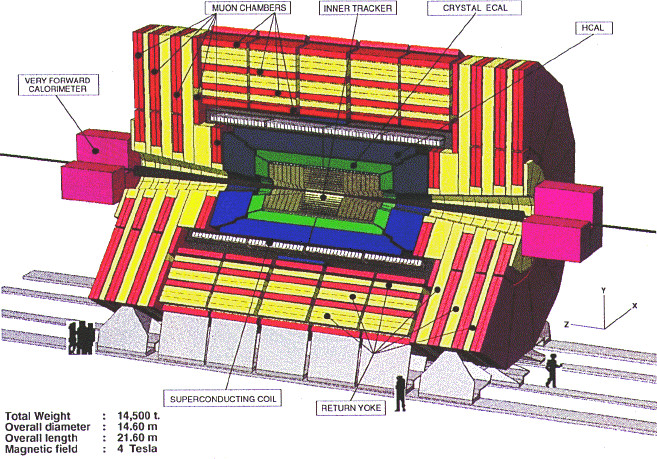
\includegraphics[width=4in]{images/CMSdetc3D.jpg}
  \caption
   {The CMS detector \cite{cmsweb}}
  \label{fig:cmsdet3d}
\end{figure}

CMS was built primarily to look for the Standard Model Higgs and signs of Beyond Standard Model (BSM) physics like Supersymmetry, extra dimensions, or new heavy weak bosons \cite{tdr}. Because BSM and Higgs decays to muons and electrons often have the highest signal to background ratio, CMS is designed to identify and measure these particles with a high accuracy. In layman's terms a high signal to background ratio just means that these events have fewer look-alikes. Jets \footnote{When a quark or gluon is created it can't exist alone, since it has color charge, and pulls other quarks from the vacuum creating a tight cone of composite colorless particles as well as their decays. This cone of particles is called a jet.} and photons are measured to a high degree of accuracy as well. In order to measure the energy, momentum, and location of the different types of particles CMS deploys a variety of subdetectors working in concert. The defining feature of the detector is an extremely powerful solenoid which enables the accurate measurement of momentum for charged particles. The tracker and calorimeters fit snugly within the 6 m diameter solenoid. The muon detectors reside outside the magnet but within the return yoke.

\subsection{Silicon Tracker}
The 3.8T magnetic field inside the solenoid enables the tracker to measure the transverse momentum of charged particles based upon the curvature of the track. Charged particles with lower transverse momentum ($p_{t}$) bend more in a magnetic field than high $p_{t}$ particles. As such, a measurement of the deviation of a curved track from a straight line, the sagitta, can be used to measure the curvature and determine the momentum \cite{pdgreview}.

\begin{equation}
p_{t} \cong \frac{L^{2}qB}{8s}
\end{equation}

Here L is the length of the straight line between the first and last position measurments, q is the charge of the particle, B is the magnetic field, and s is the sagitta.

\begin{figure}[h!]
  \centering
  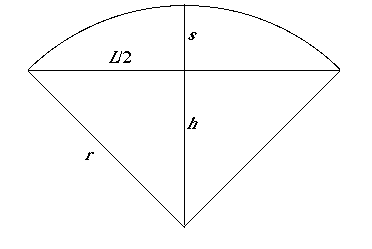
\includegraphics[width=3in]{images/sagitta.png}
  \caption
   {The sagitta measurement}
  \label{fig:sagittadrawing}
\end{figure}

The equation for the error in the momentum measurement shows that a higher magnetic field enables better $p_{t}$ resolution, illuminating the design choice for a powerful magnet.

\begin{equation}
\frac{\delta p_{t}}{p_{t}} \propto \frac{p_{t}}{L^{2}B} 
\end{equation}

The silicon tracker is made of tiny reverse biased bipolar diodes. When a charged particle travels through one of these diodes the ionization force of the particle releases electron hole pairs beyond the electrostatic equilibrium, inciting a current to flow. The tracker needs to be small enough such that the particles flowing through it don't deposit much energy. Energy deposition in the tracker would throw off energy measurements in the calorimeters. This means that the tracker needs to be smaller than a few radiation lengths \footnote{the length scale over which an electron deposits a substantial amount of energy into the material}. The tracker at the thickest part is one radiation length. The tracker is placed nearest the collision point in order to identify primary and secondary vertices and to measure the momentum of particles before they are tainted by interactions with other detectors. \footnote{Vertex is shorthand for the location of the collision or decay that produced a set of particles.} Being so near the collision point, the silicon tracker is bombarded by a constant flux of high intensity radiation. As such, the tracker is carefully designed to be robust to this radiation rich environment.

\subsection{Calorimeters}
The Electromagnetic Calorimeter (ECAL) is right outside the tracker and its main goal is to measure the energy of electrons and photons. It's designed to contain entire electromagnetic showers for these particles and is consequently many radiation lengths thick. The ECAL is made of lead tungstenate scintillating crystals which release an amount of light proportional to the energy deposition. The light is collected and the total energy is calculated. The separation into individual crystals allows some spatial resolution as well. Particles with larger mass deposit less energy per unit distance into a solid. Many of the hadronic particles make it through the ECAL for this reason.

\begin{figure}[h!]
  \centering
  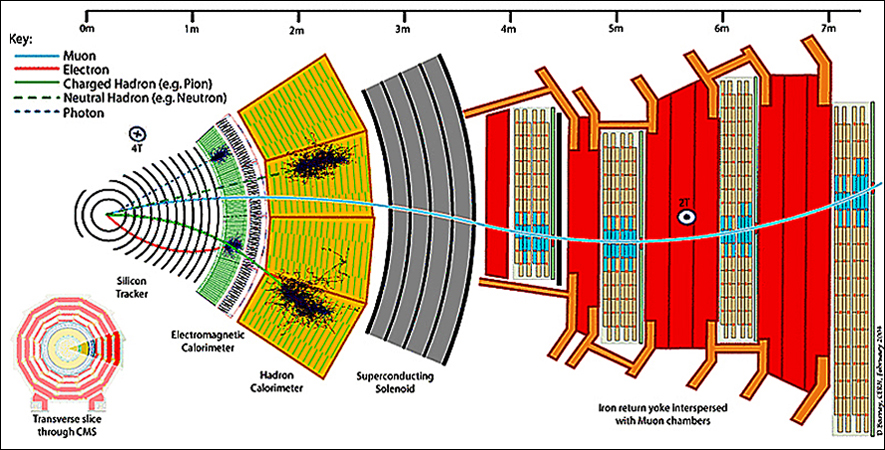
\includegraphics[width=4in]{images/cms_slice.jpg}
  \caption
   {A slice of the CMS detector \cite{cmsweb}}
  \label{fig:cmsdetslice}
\end{figure}

The HCAL is placed outside the ECAL to collect the energy of the particles that survived the other subsystems, mostly strongly interacting hadronic particles from jets. The HCAL works in a similar manner to the ECAL except that layers of plastic scintillating material are interspersed with layers of a dense passive absorber like brass or steel. The density of the passive absorber increases the chance of interaction and shower production thus reducing the total length of the hadronic shower and enabling the measurement of the total energy for most of the cascades. Again the scintillation light is collected to determine the energy. If the ECAL and HCAL were placed outside the magnet the particles would interact with the solenoid material before entering the calorimeters, throwing off their measurements. The showers in the calorimeters are a consequence of the electromagnetic and strong forces, which means that particles without these interactions pass through the materials undetected, e.g. neutrinos or BSM weakly interacting particles. Since the momentum in an interaction is conserved any imbalance means that some particles escaped the detector. If there is an excess of missing momentum beyond the amount expected due to neutrinos this may indicate the existence of dark matter or some other BSM particle. In order to measure the missing energy correctly it's important that the HCAL is built without any gaps and that it is dense enough to collect the energy of the strongly and electrically interacting particles.

While the momentum resolution in the tracker is proportional to the momentum, the energy resolution in the calorimeters decreases with increasing energy \cite{pdgreview}.

\begin{equation}
\frac{\delta E}{E} = \sqrt{\left(\frac{S}{\sqrt{E}}\right)^2 + \left(\frac{N}{E}\right)^2 + C}
\end{equation}

The first term in the square root describes statistical fluctuations. The energy measured is proportional to the number of photons captured which has poisonnian fluctuations and the error (${\rm \delta E}$) for this term is $\propto \sqrt{{\rm E}}$. The second term describes noise in the electronics whose error is energy independent, and the last term describes the errors in energy calibration which are proportional to energy.

\subsection{Muon System}
Neutrinos aren't the only Standard Model particles that make it through the tracker, ECAL, and HCAL. Muons have a relatively long lifetime $\sim 10^{-6} s$  with $c\tau \sim 100 m$. The large gamma factor in combination with their long lifetime enables them to travel hundreds of kilometers on average, well through the entire CMS detector before decaying. Muons are charged so their tracks show up in the tracker and some energy is deposited in the calorimeters but, muons are so much more massive than electrons that the energy deposition in the ECAL is minimal. Making it through the ECAL the muons enter the HCAL. The HCAL is designed to stop strongly interacting hadronic particles and collect their energy. But muons don't interact with the strong force and make it through the HCAL as well. This enables the muon system to be placed outside the magnet.

The muon system consists of a few different types of detectors which all involve the same basic principle. The charged muon ionizes some gas and the ionized particles are attracted to charged surfaces initiating a current in the surfaces. With a large enough voltage differential between the charged surfaces the the ionized particles may gain enough kinetic energy to further ionize other atoms in the gas initiating an avalanche effect and reducing the need for signal amplification later. The muon system uses this strategy in the different detectors. The types of detectors in the muon system are the Cathode Strip Chambers (CSC), the Drift Tubes (DT), and the Resistive Plate Chambers (RPC) \cite{tdr}.

\begin{figure}[h!]
  \centering
  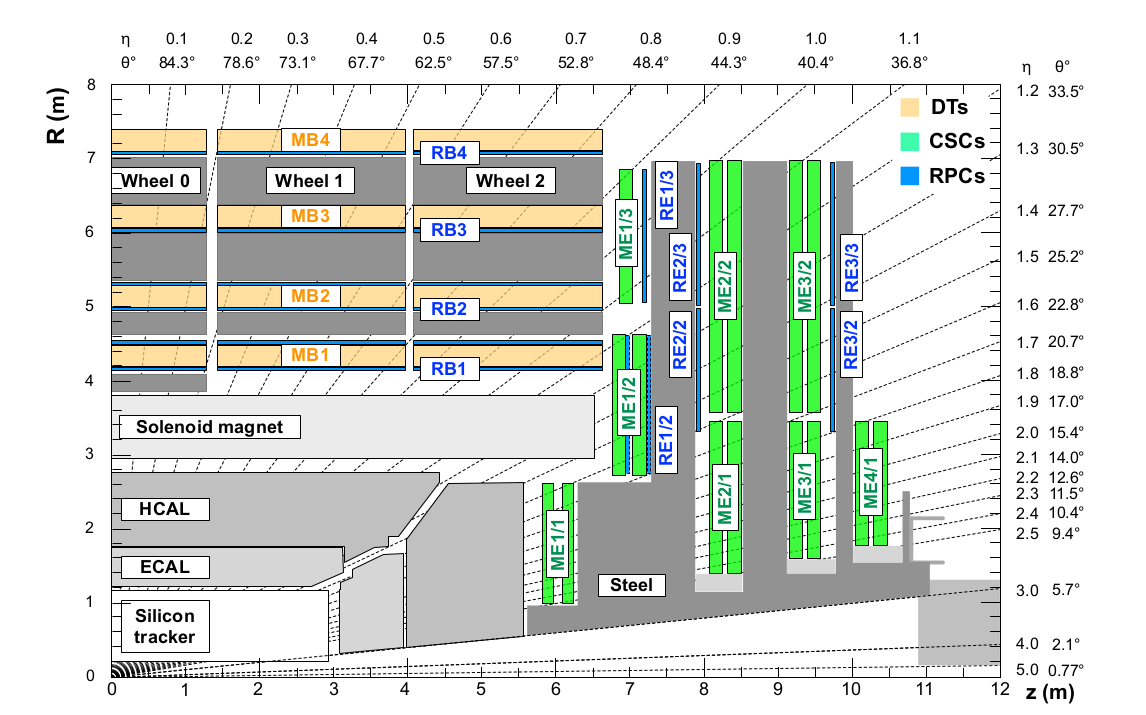
\includegraphics[width=5.5in]{images/muon_system.png}
  \caption
   {A Look at the Muon System \cite{muonsys}}
  \label{fig:muonsysfig}
\end{figure}

\newpage

\subsubsection{Drift Tubes}

The drift tubes are located in the barrel portion of CMS. Throughout the majority of the barrel the magnetic field is basically uniform. The drift tubes have aluminum plates on the top and bottom separated by aluminum I-beams shown in Figure ~\ref{fig:dt}. A wire acts as the anode and the I-beams are the cathodes. The tubes are designed to provide a constant drift velocity throughout each tube.

\begin{figure}[h!]
  \centering
  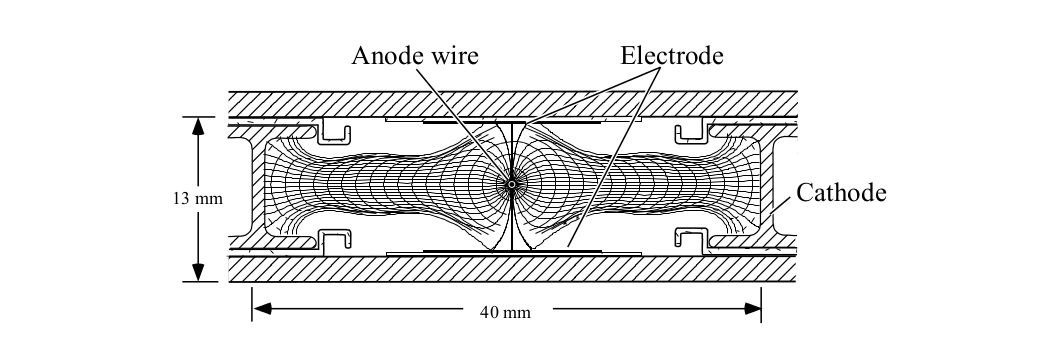
\includegraphics[width=4in]{images/DT.png}
  \caption
   {A Drift Tube \cite{mutdr}}
  \label{fig:dt}
\end{figure}

When a charged particle flies through the tube it ionizes the gas inside. The electrons drift at constant velocity to the anode. The distance from the anode is deduced from the drift time, utilizing the fact that the ionized electrons drift with a constant velocity. This calculation does however require a reference time. In each chamber the drift tubes are placed in layers and the average crossing time in the chamber is used as the reference time.

\subsubsection{Cathode Strip Chambers}

The CSCs are located in the endcaps of the detector which range in $|\eta|$ from 0.8 to 2.4. One of the reasons the endcaps use CSCs instead of DTs is the nonuniform magnetic field which would adversely affect the drift times in the DT system. In this system there are oppositely charged strips and wires running roughly perpendicular to eachother.

\begin{figure}[h!]
  \centering
  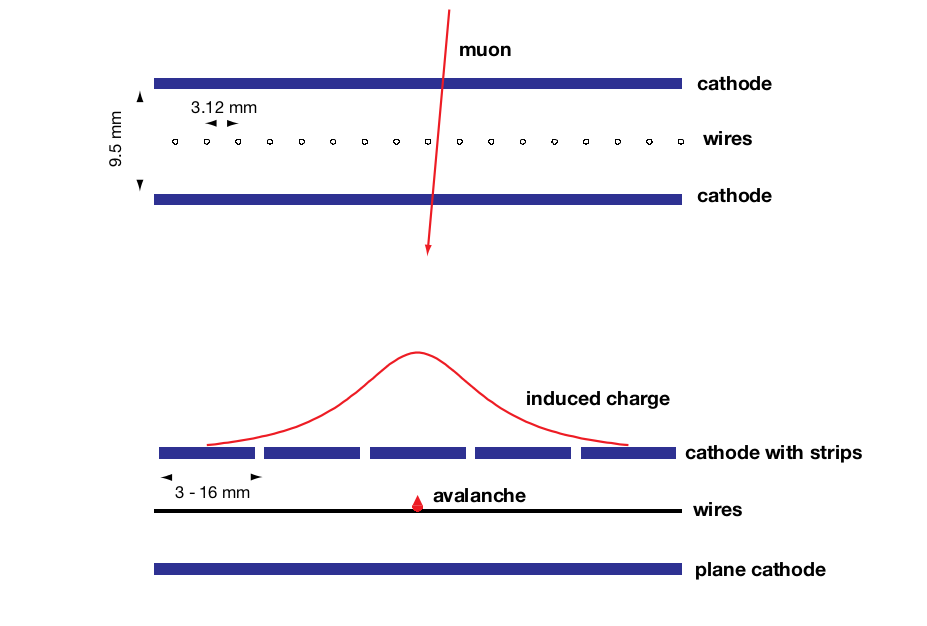
\includegraphics[width=4in]{images/CSC.png}
  \caption
   {A Cathode Strip Chamber \cite{mutdr}}
  \label{fig:csc}
\end{figure}

When a muon flies through the CSC it induces charge on the wires and the strips and ionizes gas in the chamber. The ionized particles in the gas float to the charged strips and wires initiating a current in the nearby wires and strips. The induced charge from the muon itself also contributes to the currents. The most intense currents should be those associated with the location of the muon. The position resolution in the phi direction is roughly 100 ${\rm \mu m}$.

\subsubsection{Resistive Plate Chambers}

The RPCs are located both in the barrel and in the end caps. The RPCs have excellent timing resolution on the order of 1 ns. The RPCs use their excellent timing resolution to determine each particle's bunch crossing of origin. The accurate and rapid timing information helps with the online selection of muons, a huge priority for CMS considering that many interesting collisions produce muons. For this reason the RPCs focus on efficient online selection of muons instead of accurate offline reconstruction \cite{cmsexp}.

In this way the RPCs complement the DTs and CSCs. The RPCs consist of two high resistance parallel plates surrounding a volume of gas. The outsides of the plates are painted with graphite paint forming the electrodes. A large voltage differential is kept between the electrodes. When a charged particle crosses the plates it induces an electrical discharge in the plates which remains localized in time and space due to the large resistivity.

\subsection{Trigger System}
Collision events come at a rate of 10 MHz with each event taking up roughly a MB of information. If the detector had to store all of the information from each event this would amount to pushing terabytes of information into a storage system every second, which is remarkably infeasible. To deal with this issue CMS utilizes a trigger system, which selects only interesting events cutting the rate down from 10 MHz to 1 KHz \cite{cmsexp}. Since bunch crossings happen every 25 ns the trigger needs to operate at an incredibly high rate.

CMS tackled this issue by dividing the trigger into different tiers. The Level 1 Trigger is the first stage of the trigger system made from custom hardware which can operate at fantastic speed. The Level 1 Trigger reduces the rate from 10 MHz to 100 KHz and the events passing the L1 Trigger go onto the High Level Trigger (HLT) which further reduces the rate to 1 KHz. Due to the lower input rate the HLT can operate in software.

\subsubsection{L1 Trigger}

The L1 Trigger is made of up different subsystems that work together to decide whether to keep the data from a beam crossing for further processing. The University of Florida works with the Level 1 muon trigger system, the Endcap Muon Track Finder (EMTF) in particular. The muon system needs to determine the transverse momenta of muons and their location and choose the best candidates. Each of the different muon detectors have their own local triggers which send their best muon tracks to the Global Muon Trigger (GMT). The GMT chooses the best muon candidates from that set and passes these on to the Global Trigger (GT). The GT combines the information from the calorimeter triggering system. The GT uses this combined information to check whether the bunch crossing should be sent to the HLT or discarded. The L1 Trigger has many different trigger criteria defining separate triggers which are the trigger bits. If an event passes any of the triggers then it is forwarded for further processing.

\begin{figure}[h!]
  \centering
  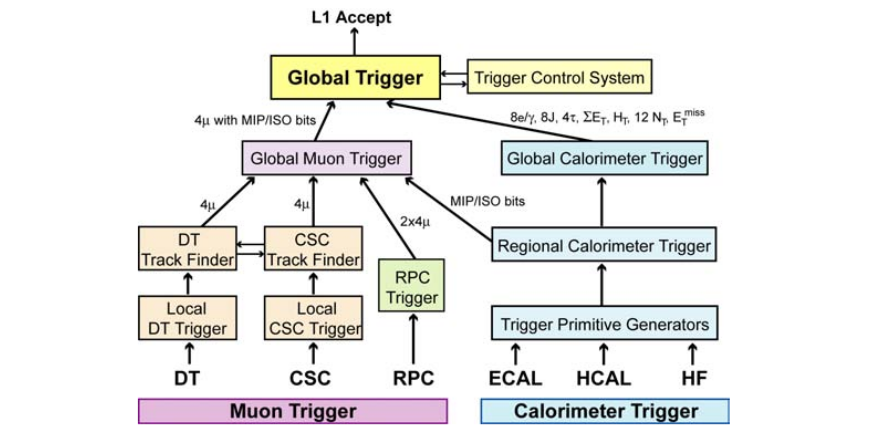
\includegraphics[width=5in]{images/L1_Trigger.png}
  \caption
   {The L1 Trigger Architecture \cite{cmsexp}}
  \label{fig:l1trigarch}
\end{figure}

The Track Finders (TF) play an important role in the L1 Trigger system. The EMTF combines the location and direction information from the different CSC stations into muon tracks and calculates the transverse momenta for the different tracks. The EMTF chooses the best candidates (highest momentum and highest quality) to send to the GMT. The Drift Tube Track Finder (DTTF) performs a similar process for muons in the DT system. The RPC system calculates the location and direction and forms tracks in the same stage. In the process the RPC trigger system assigns transverse momenta and quality, and like the others chooses the best tracks to send to the GMT.

\chapter{THE STANDARD MODEL} \label{sm}

The Standard Model (SM) of particle physics is an incredibly successful theory that correctly describes the physics of all known particles and forces that make up the universe, excluding gravity \cite{smconsistency}. The particles of the SM come in two types, fermions and bosons \footnote{Bosons have integer spin.}. Fermions are the spin 1/2 particles and make up the different types of matter. Electrons are a familiar example, and the up and down quarks that make up protons and neutrons are others. While electrons and the up and down quarks account for nearly all of the matter in our day to day experience there are actually many other fermions. In fact, there are three generations of quarks and leptons \footnote{Leptons are fermions that aren't quarks.} with each generation heavier than the next. The up and down quarks are the first generation of quarks, charmed and strange are the next, and top and bottom are the third generation. For the leptons the electron and electron neutrino are the first generation, the muon and muon neutrino are the second, and the tau and the tau neutrino the third. Each fermion also has a corresponding antiparticle. As an example, the positron is the antiparticle for the electron. 

\begin{figure}[h!]
  \centering
  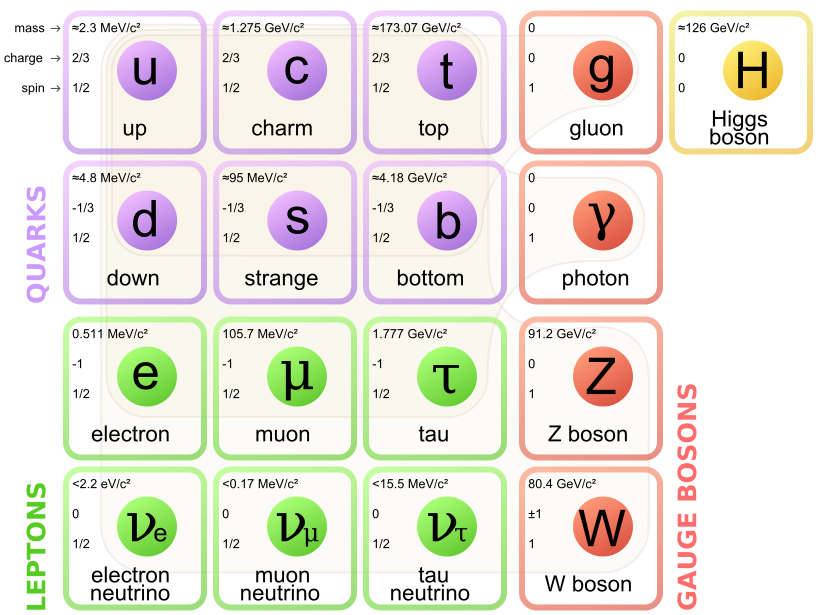
\includegraphics[width=4in]{images/Standard_Model_of_Elementary_Particles.png}
  \caption
   {The Standard Model Particles}
  \label{fig:smtable}
\end{figure}

The universe would be pretty boring if the particles couldn't attract or repel or form more complex objects like atoms, molecules, and even people. Luckily there are forces as well and these forces are described by the spin 1 bosons. The fermions attract and repel by exchanging bosons, which is why the bosons are often called force carriers. Gluons mediate the strong force, photons the electromagnetic force, and the W and Z bosons mediate the weak force. Every force has an associated charge. Just as those particles with electric charge can interact through the electromagnetic force, those with color charge may interact via the strong force, and those with isospin may interact through the weak force. The fundamental forces and particles interact to make the familiar composite objects that surround us in our daily lives. The strong force binds quarks to form protons and neutrons, the Van Der Waals version of the strong force binds the protons and neutrons together to form nuclei, and the electromagnetic force binds electrons and nuclei to form atoms. The size of the composite objects gives an idea of the relative strength of the forces. A proton is ~$10^-15$ meters in size while an atom is ~$10^-10$ meters and a solar system is ~$10^12$ meters. The more tightly bound the stronger the force. In fact the ratio of the strength of the forces is like so 1:$10^-3$:$10^-16$:$10^-41$, strong : electromagnetic : weak :gravitational \footnote{Gravity is just included for perspective. The Standard Model does not describe this force and reconciling gravity with quantum mechanics is an open problem.}. 

Of all the particles predicted by the SM, only the Higgs boson remains to be found. The Higgs boson is the only spin 0 particle of the SM. It is theorized that as the universe cooled from the Big Bang the Higgs field went through a phase transition and settled into a nonzero ground state forming a condensate. And it is the potential energy from the interactions with this nonzero ground state that give the massive fundamental particles their mass. With such a large role in the SM, finding this particle or a BSM Higgs has been a huge priority for the CMS collaboration \cite{tdr}. In 2012 a Higgs particle with a mass of 125 GeV was found and to date remains consistent with the Standard Model. However, the properties need to be investigated further before declaring the discovered Higgs the Higgs of the Standard Model. 


%%%%%%%%%%%%%%%%%%%%%%%%%%%%%%%%%%%%%%%%%%%%%%%%%%%%%%%%%%%%%%%%%%%%%%%%%%%

\section{Quantum Field Theory}


The mathematical framework used to describe the physics of the SM as well as other Beyond Standard Model (BSM) field theories is called Quantum Field Theory (QFT). QFT enables the predictions of measurable quantities, namely the probabilities for different sets of particles to come out of a specific collision or for a single particle to decay into different sets of particles. These probabilities are encompassed in the cross sections and branching fractions. For example, the theory of the SM predicts the cross section for two protons colliding and making a Higgs. As another example, the SM also predicts the branching fraction for a Z boson decaying to two muons. These probabilities can be measured simply by colliding particles and counting the outcomes which in turn means that the theory can be tested. In fact, any QFT model can be tested in this manner. There are other commonly measured properties as well like the lifetime, spin, and mass of different particles.  

\subsection{What is a Particle?}

Since QFT makes quantitative predictions in terms of particle collisions and particle decays it's interesting to contemplate what a particle really is. The idea of a particle is often taken for granted. Consider an observer in a frame x with particle p and an observer in another frame x'. If the observer in x' can't identify particle p then it doesn't make sense to call p a particle. More concretely, consider a world where in frame x an observer sees a neatly stacked deck of cards, but in x' the observer sees the cards scattered all over the place. Calling the deck of cards a particle doesn't really make sense. On the other hand, both parties can still agree on the individual cards which kept the same suit and value. These are conserved quantities. If the two observers get together later and compare notes they can see what happened to each card upon transforming from x to x' and work out a set of rules. The king of hearts may do one thing and the 10 of clubs another. They can then add the different forces into play repeat the process and compare again. Figuring this all out determines the laws of physics for the fundamental pieces called particles.       

This idea leads to Wigner's view: a particle is an object with conserved quantities that observers can agree on between frames. In our universe these labels are the mass, charge, spin, color, and isospin. And because different observers can agree on these quantities they can compare notes and work out the laws of physics for the different types of particles. All that remains is to work out laws that people in different frames can confirm, and this is where the Lagrangian formalism comes into play. 

\subsection{The Lagrangian Formalism}

The Lagrangian formalism is a mathematical device that allows physicists to describe the evolution of a physical system over time, and it's within this formalism that QFT can be built. But before building the full mathematics of QFT, a simple example of the free Newtonian particle is given, and the different symmetries are observed. The Newtonian example serves as a starting point, and eventually the theory of the Standard Model will be developed using the symmetries as a roadmap. The fact that the laws of physics are indistinguishable in different inertial frames along with the requirement that the speed of light remain constant in all frames of reference lay the foundation for QFT. 

So let's get into the framework. The goal of physics is to describe how a physical system evolves over time, and this evolution is usually given by some differential equation describing the state the system will take in the next interval of time given the current time. Moving from state to state from one interval of time to the next, the system traces out a path in space and time or some other more abstract space of possible states. So how does one get the appropriate differential equation? As it turns out nature tries to minimize the difference between the energy spent \footnote{Spent here just means used as kinetic energy.} and the energy available to spend and it minimizes the action S. In the equation below, L is the Lagrangian, T is the kinetic energy and U is the potential energy.     
\begin{equation}
S = \int L dt = \int T - U dt
\end{equation}

At an extremum of S, $\delta S$ = 0 since S must go down then through a slope of zero and back up or vice versa. This assumes continuity and must be true for all parameters -- all directions. So to get the equations of motion just vary the parameters of L and solve for the values that yield zero change in the action.

\begin{equation}
\delta S = \int L(z_1 + dz_1, z_2+dz_2, ...)dt - \int L(z_1, z_2, ...)dt 
\end{equation}

Following this process yields the Euler-Lagrange (differential) equations, describing how the parameters z evolve over time. The z's may be the position and velocity, or the quantum fields, or the temperature and volume or some other set of parameters that describe the system. The Lagrangian for a Newtonian free particle in one dimension is pretty simple and gets the point across. 

\begin{equation}
S = \frac{1}{2} \int m\dot{x}^2 dt
\end{equation}

If the action is at an extremum, perturbing the path x(t) by adding the infinitesimal $\epsilon$(t) leaves the action unchanged.

\begin{equation}
S' = \frac{1}{2} \int m(\dot{x} + \dot{\epsilon})^2 dt = \frac{1}{2} \int m(\dot{x}^2 + 2\dot{x}\dot{\epsilon} + \dot{\epsilon}^2) dt =  
\frac{1}{2} \int m(\dot{x}^2 + 2\dot{x}d\dot{x}) dt 
\end{equation}

\begin{equation}
\delta S = S' - S = 0 = \frac{1}{2} \int m(\dot{x}^2 + 2\dot{x}\dot{\epsilon}) dt - \frac{1}{2} \int m\dot{x}^2 dt = \int m\dot{x}\dot{\epsilon} dt
\end{equation}

Since x(t) is fixed at the boundaries of the integral, $\epsilon$ must be zero at $t_o$ and $t_f$, so integrating by parts yields the following equation. 

\begin{equation}
\delta S = 0 = \epsilon(t_f) \dot{x}(t_f)  - \epsilon(t_o) \dot{x}(t_o) + \int m\ddot{x} \epsilon dt  = 
0\dot{x}(t_f)  - 0\dot{x}(t_o) + \int m\ddot{x} \epsilon dt = \int m\ddot{x} \epsilon dt
\end{equation}

And this equation must be zero for any infinitesimal deviation $\epsilon$.

\begin{equation}
\delta S = 0 \rightarrow m\ddot{x} = 0
\end{equation}

So a free particle keeps the same velocity over time. Note that a Newtonian boost by constant velocity $v \rightarrow v' = v + u$ \footnote{Renaming $\dot{x}$ as v.} leaves the equations of motion consistent. In the unprimed frame the particle has velocity v with 0 acceleration. In the primed frame the particle has velocity v + u with 0 acceleration. Both observers see the particle act as if there are zero forces.

\begin{equation}
S = \frac{1}{2} \int m(v + u)^2 dt  =  \frac{1}{2} \int m(v')^2 dt \rightarrow \delta S = 0 \rightarrow m\frac{d}{dt}(v+u) = m\frac{d}{dt}(v') = 0 
\end{equation}

If u is not constant but a function of time u(t) then the equations of motion do not describe the same time evolution.

\begin{equation}
m\frac{d}{dt}(v+u) = m\dot{v} + m\dot{u} = 0 \rightarrow \dot{v} = -\dot{u}
\end{equation}

In the case where u(t) depends upon time, the difference between the primed and unprimed frames' equations of motion is then $\delta F$.

\begin{equation}
\delta F = m\frac{d}{dt}(v+u) - m\frac{dv}{dt} = m\dot{v} + m\dot{u} - m\dot{v} = m\dot{u}
\end{equation}

In the unprimed frame, the particle identified by the mass moves with constant velocity, $\dot{v} = 0$. The observer in the primed frame looks at the particle with the same mass and sees it change velocity given by the equation $\dot{v} = -\dot{u}$. As an example, set v and $u, \dot{u}$ to zero for all times before t=0, and let $u, \dot{u}$ turn on after time 0. Both observers will agree that the particle is stationary up until time 0. After which, the observer in the primed frame will see the particle accelerate in strange ways. Meanwhile, the unprimed frame will continue to observe a stationary particle. 

In general, every inertial frame finds $\delta F = 0$ and every accelerating frame finds an extra force $\delta F$ unique to its acceleration. In this way no observer in an inertial frame can perform an experiment and determine which inertial frame he or she is in. On the other hand, each accelerating frame is identified by its $\delta F$.  In every inertial frame a ball released at rest remains at rest. In an accelerating frame the ball will accelerate according to the motion of the frame $\delta F$ and this change in the laws of physics identifies the frame in a unique way. Conversely, the laws of physics remain the same boosting between inertial frames, and this invariance is a symmetry of physics. Of course this example is Newtonian and the correct way to boost is given by the Lorentz transformation from Special Relativity, but this gets the point across.

Delving further along the path of symmetry, the fundamental forces depend only on the distance from the charge and not the direction implying that rotations are also a symmetry. This can be seen by looking at the Lagrangian. 

\begin{equation}
L = \frac{1}{2} m\dot{\vec{x}}^2 - U((\vec{x} - \vec{x'})^2)
\end{equation}

Rotations leave dot products and consequently the magnitude of vectors unchanged so the Lagrangian is invariant under this transformation. Naturally if the Lagrangian is invariant the equations of motion will be as well.

\begin{equation}
m\frac{d\vec{v}}{dt} = \vec{\nabla} U
\end{equation}

In the equations of motion above, both sides are vectors and vectors transform the same way under rotations so the equations of motion are invariant. Note that in the case of rotations both the Lagrangian and the equations of motion are invariant. While for Newtonian boosts only the equations of motion were invariant. This is due to the fact that Newtonian mechanics is the low velocity limit of relativistic mechanics. In the theory of Special Relativity the action for a massive free particle is written like so.

\begin{equation}
S = \int \frac{m}{2}u^{\mu}u_{\mu}d\tau
\end{equation}

Just as rotations preserve the dot product, Lorentz transformations (boosts and rotations) preserve the four vector product. Insofar, both the relativistic Lagrangian and the resulting equations of motion remain invariant under a boost or rotation to a new inertial frame. Building the Lagrangian out of four vector products gaurantees this. Interestingly enough, by studying the properties of the Lorentz group it's possible to find even more fundamental building blocks called spinors.

\subsection{QFT From Symmetry}

The laws of physics are invariant under boosts and rotations, and the Lagrangian provides a mathematical framework for physical predictions. These facts together imply that there's a good shot at building a proper QFT by creating the appropriate invariant Lagrangian. Four vector products remain invariant under Lorentz transformations so they are a natural ingredient, but there are other mathematical objects that could be used as well. In this vein, the symmetries under rotations and boosts are investigated in order to look for some other building blocks. The goal is to find two different representations of the Lorentz group and use one representation to describe fermions and other for bosons.

\subsubsection{Rotations}

Rotations in three dimensions are described by the SO(3) group. Rotations preserve the lengths of vectors and the angles between them, which means that dot products between vectors remain invariant as well. In three dimensions one can rotate about any of the three axes. The rotations about the x, y, and z axes may be characterized by the matrices below.

\begin{equation}
R_x = 
\begin{pmatrix}
1 & 0 & 0 \\
0 & \cos\theta_x & -\sin\theta_x \\
0 & \sin\theta_x & \cos\theta_x \\
\end{pmatrix}
\end{equation}

\begin{equation}
R_y = 
\begin{pmatrix}
\cos\theta_y & 0 & \sin\theta_y \\
0 & 1 & 0 \\
-\sin\theta_y & 0 & \cos\theta_y \\
\end{pmatrix}
\end{equation}

\begin{equation}
R_z = 
\begin{pmatrix}
\cos\theta_z & -\sin\theta_z & 0 \\
\sin\theta_z & \cos\theta_z & 0 \\
0 & 0 & 1 \\
\end{pmatrix}
\end{equation}

These rotations may be built up from repeated rotations by an infinitesimally small angle $d\theta$. The matrices characterizing an infinitesimal rotation are given by taking the limit as $\theta$ goes to zero.

\begin{equation}
dR_x = 
\begin{pmatrix}
1 & 0 & 0 \\
0 & 1 & -d\theta_x \\
0 & d\theta_x & 1 \\
\end{pmatrix}
= 1 - id\theta_x
\begin{pmatrix}
0 & 0 & 0 \\
0 & 0 & -i \\
0 & i & 0 \\
\end{pmatrix}
= 1 - id\theta_x J_x
\end{equation}

\begin{equation}
dR_y = 
\begin{pmatrix}
1 & 0 & d\theta_y \\
0 & 1 & 0 \\
-d\theta_y & 0 & 1 \\
\end{pmatrix}
= 1 - id\theta_y
\begin{pmatrix}
0 & 0 & i \\
0 & 0 & 0 \\
-i & 0 & 0 \\
\end{pmatrix}
= 1 - id\theta_y J_y
\end{equation}

\begin{equation}
dR_z = 
\begin{pmatrix}
1 & -d\theta_z & 0 \\
d\theta_z & 1 & 0 \\
0 & 0 & 1 \\
\end{pmatrix}
= 1 - id\theta_z 
\begin{pmatrix}
0 & -i & 0 \\
i & 0 & 0 \\
0 & 0 & 0 \\
\end{pmatrix}
= 1 - id\theta_z J_z
\end{equation}

Repeating an infinitesimal rotation many times rebuilds the finite rotation, so the J matrices generate rotations along their respective axes and they are aptly referred to asthe generators of the group. Some algebra reveals this to be the case.

\begin{equation}
R = (1 - i\frac{\theta}{N} J)^{N} = 1 + (-id\theta J) + \frac{1}{2!}(-id\theta J)^2 + \frac{1}{3!}(-id\theta J)^3 + ... = e^{-i\theta J} 
\end{equation}

Notice that even powers of J yield $J^2$ and that odd powers of J return J.

\begin{equation}
  = 1 - J^2 + J^2(1 + \frac{i^2}{2!} d\theta^2 + \frac{i^4}{4!} d\theta^4 + ...) - iJ(d\theta + \frac{i^2}{3!}d\theta^3 + \frac{i^4}{5!}d\theta^5 + ...) 
  = (1-J^2) + J^2 \cos\theta - iJ\sin\theta
\end{equation}

Plugging in $J_z$ reveals that this process does in fact rebuild the rotation matrix $R_z$.

\begin{equation}
\begin{split}
R_z &= 
(\begin{pmatrix}
1 & 0 & 0 \\
0 & 1 & 0 \\
0 & 0 & 1 \\
\end{pmatrix}
-
\begin{pmatrix}
1 & 0 & 0 \\
0 & 1 & 0 \\
0 & 0 & 0 \\
\end{pmatrix})
+
\begin{pmatrix}
1 & 0 & 0 \\
0 & 1 & 0 \\
0 & 0 & 0 \\
\end{pmatrix}
\cos\theta_z
+
\begin{pmatrix}
0 & -1 & 0 \\
1 & 0 & 0 \\
0 & 0 & 0 \\
\end{pmatrix}
\sin\theta_z
\\ &=
\begin{pmatrix}
\cos\theta_z & -\sin\theta_z & 0 \\
\sin\theta_z & \cos\theta_z & 0 \\
0 & 0 & 1 \\
\end{pmatrix}
\end{split}
\end{equation}

Similarly, the other generators rebuild their respective rotation matrices. The generators of the group are actually more fundamental than the rotation matrices. The multiplication table for the generators describes the algebra of the group, which describes the behavior of rotations at a local level. In fact the rotation matrices are just one of the groups with this local algebra, and a specific group obeying the local algebra is analagous to a specific solution of a differential equation: each solution has a different global behavior yet each obeys the same physics. Moreover the multiplication table can be specified without declaring any particular representation for the generators. 

\begin{equation}
\begin{split}
&J_x*J_y = iJ_z  + J_y*J_x \\
&J_y*J_z = iJ_x  + J_z*J_y \\
&J_z*J_x = iJ_y  + J_x*J_z \\
\end{split}
\end{equation}

The multiplication table can be specified in a more compact notation using the commutator, $[a,b] = ab - ba$, and the antisymmetric tensor $\epsilon$.
\begin{equation}
[J_k, J_l] = i\epsilon_{klm}J_m
\end{equation}

Finding 3x3 generators that obey the algebra and then repeatedly applying the infinitesimal transormations builds the SO(3) rotation group. The group acts on 3x1 objects called vectors, and these 3x1 vectors are a suitable candidate for a Newtonian Lagrangian. Finding another representation obeying this algebra will provide a more fundamental ingredient for the Lagrangian and allow the construction of a proper QFT. Similar to the way real numbers are built from the squares of imaginary numbers, vectors are built from spinors. 

Looking for the lowest order complex nxn matrices satisfying the algebra gives the 2x2 Pauli matrices. Any 1x1 matrices are simply scalar complex numbers, which commute and therefore cannot satisfy the algebra. The Pauli matrices are  

\begin{equation}
\sigma_x = 
\begin{pmatrix}
0 & 1 \\
1 & 0 \\
\end{pmatrix},
\sigma_y = 
\begin{pmatrix}
0 & -i \\
i & 0 \\
\end{pmatrix},
\sigma_y = 
\begin{pmatrix}
1 & 0 \\
0 & -1 \\
\end{pmatrix}
\end{equation}

However, plugging these into the commutator reveals a factor of two difference.

\begin{equation}
[\sigma_k, \sigma_l] = 2i\epsilon_{klm}\sigma_m
\end{equation}

Defining $J_k = \frac{1}{2} \sigma_k$ fixes this. These matrices act on an array of 2x1 complex numbers called spinors, and this new "rotation" group is called SU(2). Note that by starting with vectors and analyzing the SO(3) rotation group along with its underlying algebra, new mathematical objects have been discovered. It's now possible to use these spinors to build rotationally invariant Lagrangians. While rotationally invariant Lagrangians are important for nonrelativistic theories, the real goal is to break down four vectors in the same way to find the most fundamental ingredients for relativistic Lagrangians. 

\begin{equation}
[J_k, J_l] = i\epsilon_{klm}J_m
\end{equation}

\subsubsection{The Lorentz Group}
Four vector products are invariant with regards to rotations and boosts. This statement is defined by the mathematical equation below, where the $\Lambda$ matrices represent the rotation/boost matrices of the Lorentz Group and the $\eta$ matrix is the Minkowski metric $\left( \begin{smallmatrix} 1 & 0 & 0 & 0 \\ 0 & -1 & 0 & 0 \\ 0 & 0 & -1 & 0 \\ 0 & 0 & 0 & -1 \\ \end{smallmatrix} \right)$.

\begin{equation}
x'_{\mu} x'^{\mu} = x_{\mu} x^{\mu} \rightarrow \eta_{\sigma\rho} \Lambda^{\sigma}_{\mu}  \Lambda^{\rho}_{\nu} x^{\mu} x^{\nu} = \eta_{\mu\nu} x^{\mu} x^{\nu}
\rightarrow \eta_{\sigma\rho} \Lambda^{\sigma}_{\mu}  \Lambda^{\rho}_{\nu} = \eta_{\mu\nu}
\end{equation}

In this 3 + 1 dimensional space the rotations and their corresponding generators are now given by the following R and J matrices.

\begin{equation}
R_x = 
\begin{pmatrix}
1 & 0 & 0 & 0\\
0 & 1 & 0 & 0 \\
0 & 0 & \cos\theta_x & -\sin\theta_x \\
0 & 0 & \sin\theta_x & \cos\theta_x \\
\end{pmatrix},
J_x = 
\begin{pmatrix}
0 & 0 & 0 & 0\\
0 & 0 & 0 & 0 \\
0 & 0 & 0 & -i \\
0 & 0 & i & 0 \\
\end{pmatrix}
\end{equation}

\begin{equation}
R_y = 
\begin{pmatrix}
1 & 0 & 0 & 0\\
0 & \cos\theta_y & 0 & \sin\theta_y \\
0 & 0 & 1 & 0 \\
0 & -\sin\theta_y & 0 & \cos\theta_y \\
\end{pmatrix},
J_y = 
\begin{pmatrix}
0 & 0 & 0 & 0\\
0 & 0 & 0 & i \\
0 & 0 & 0 & 0 \\
0 & -i & 0 & 0 \\
\end{pmatrix}
\end{equation}

\begin{equation}
R_z = 
\begin{pmatrix}
1 & 0 & 0 & 0\\
0 & \cos\theta_z & -\sin\theta_z & 0 \\
0 & \sin\theta_z & \cos\theta_z & 0 \\
0 & 0 & 0 & 1 \\
\end{pmatrix},
J_z = 
\begin{pmatrix}
0 & 0 & 0 & 0\\
0 & 0 & -i & 0 \\
0 & i & 0 & 0 \\
0 & 0 & 0 & 0 \\
\end{pmatrix}
\end{equation}

And the boosts are given by the following B matrices.

\begin{equation}
B_x = 
\begin{pmatrix}
\cosh\omega_x & \sinh\omega_x & 0 & 0 \\
\sinh\omega_x & \cosh\omega_x & 0 & 0 \\
0 & 0 & 1 & 0 \\
0 & 0 & 0 & 1 \\
\end{pmatrix}
\end{equation}

\begin{equation}
B_y = 
\begin{pmatrix}
\cosh\omega_y & 0 & \sinh\omega_y & 0 \\
0 & 1 & 0 & 0 \\
\sinh\omega_y & 0 & \cosh\omega_y & 0 \\
0 & 0 & 0 & 1 \\
\end{pmatrix}
\end{equation}

\begin{equation}
B_z = 
\begin{pmatrix}
\cosh\omega_z & 0 & 0 & \sinh\omega_z \\
0 & 1 & 0 & 0 \\
0 & 0 & 1 & 0 \\
\sinh\omega_z & 0 & 0 & \cosh\omega_z \\
\end{pmatrix}
\end{equation}

Looking at the differential boosts yields the generators K.

\begin{equation}
dB_x = 
\begin{pmatrix}
1 & d\omega_x & 0 & 0 \\
d\omega_x & 1 & 0 & 0 \\
0 & 0 & 1 & 0 \\
0 & 0 & 0 & 1 \\
\end{pmatrix}
= 1 + d\omega_x 
\begin{pmatrix}
0 & 1 & 0 & 0 \\
1 & 0 & 0 & 0 \\
0 & 0 & 0 & 0 \\
0 & 0 & 0 & 0 \\
\end{pmatrix}
= 1 + d\omega_x K_x
\end{equation}

\begin{equation}
dB_y = 
\begin{pmatrix}
1 & 0 & d\omega_y & 0 \\
0 & 1 & 0 & 0 \\
d\omega_y & 0 & 1 & 0 \\
0 & 0 & 0 & 1 \\
\end{pmatrix}
= 1 + d\omega_y
\begin{pmatrix}
0 & 0 & 1 & 0 \\
0 & 0 & 0 & 0 \\
1 & 0 & 0 & 0 \\
0 & 0 & 0 & 0 \\
\end{pmatrix}
= 1 + d\omega_y K_y
\end{equation}

\begin{equation}
dB_z = 
\begin{pmatrix}
1 & 0 & 0 & d\omega_z \\
0 & 1 & 0 & 0 \\
0 & 0 & 1 & 0 \\
d\omega_z & 0 & 0 & 1 \\
\end{pmatrix}
= 1 + d\omega_z
\begin{pmatrix}
0 & 0 & 0 & 1 \\
0 & 0 & 0 & 0 \\
0 & 0 & 0 & 0 \\
1 & 0 & 0 & 0 \\
\end{pmatrix}
= 1 + d\omega_z K_z
\end{equation}

As before with the rotations in three dimensions the group is defined by its multiplication table. 

\subsubsection{Building Lagrangians}
\subsection{Perturbation Theory}
\subsection{Feynman Rules}

\begin{figure}[h!]
  \centering
  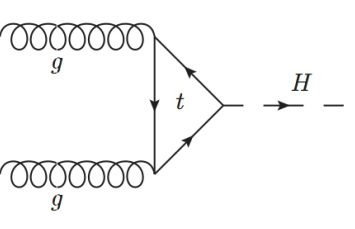
\includegraphics[width=1.5in]{images/ggf.png}
  \caption
   {The Feynman diagram for two gluons fusing into a Higgs. There are three vertices and this is a third order diagram. Two vertices involve the strong force and one vertex involves the Higgs coupling. The matrix element for this diagram would have two factors of the strong force coupling and one factor for the Higgs coupling which involves the mass of the top quark.}
  \label{fig:feynggf}
\end{figure}

%%%%%%%%%%%%%%%%%%%%%%%%%%%%%%%%%%%%%%%%%%%%%%%%%%%%%%%%%%%%%%%%%%%%%%%%%%%
\section{The Standard Model Higgs}


%%%%%%%%%%%%%%%%%%%%%%%%%%%%%%%%%%%%%%%%%%%%%%%%%%%%%%%%%%%%%%%%%%%%%%%%%%%
\subsection{SM Higgs Production and Decay Modes}

The SM Higgs can be created in a variety of ways. Some of these cross sections are shown below for 14 TeV collisions. The production cross sections are functions of the mass of the Higgs as well as the energy of the collisons. For a given collision energy the cross sections decrease as the Higgs mass increases: there are fewer kinematic possibilities for a heavier particle since more of the energy was used to create the particle. For a given mass, say 125 GeV, the cross section grows with collision energy. This constrasts with cross sections involving collisions of fundamental particles, e.g. electron antielectron collisions. This is an artifact of the fact that the LHC collides protons together. 

\begin{figure}[h!]
  \centering
  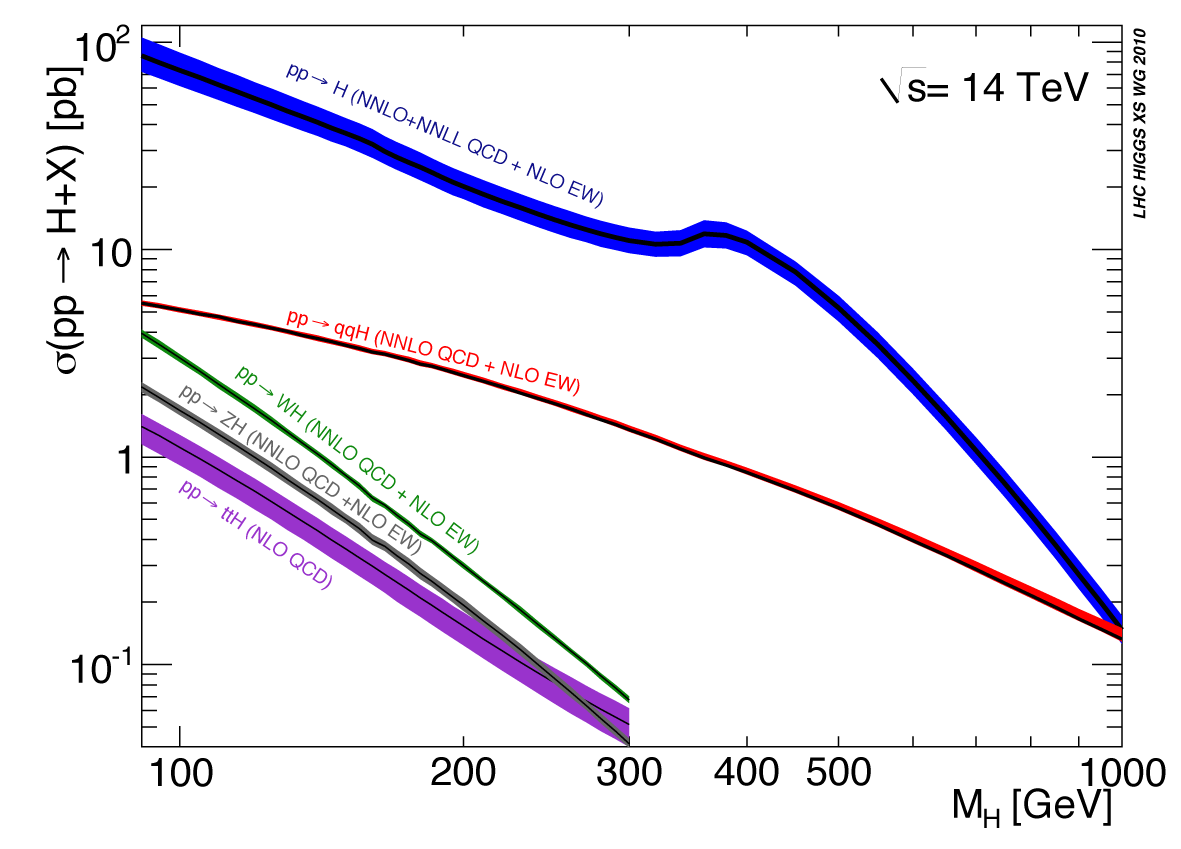
\includegraphics[width=5in]{images/14TeV_higgs_cross_sections.png}
  \caption
   {The highest production mode cross sections for the SM Higgs \cite{crossbranchplots}}
  \label{fig:hprodcross}
\end{figure}

Protons behave like a collection of an infinite number of quark-antiquarks, an infinite number of gluons, and the usual uud. The total momentum of the proton is divided up amongst them with lots of particles having little of the total momentum. The actual scattering events are between these more fundamental particles. The larger the total energy the smaller the fraction of energy needed to make a Higgs and since there are more particles with a lower fraction, this results in a growth of the cross section with collision energy. 

The SM Higgs is unstable and decays with a width of $\sim 5 MeV$ at 125 GeV. The probability of each decay changes depending upon the mass of the Higgs. In general the Higgs couples more strongly to particles with higher mass making the decays to heavier particles more likely.  

\begin{figure}[h!]
  \centering
  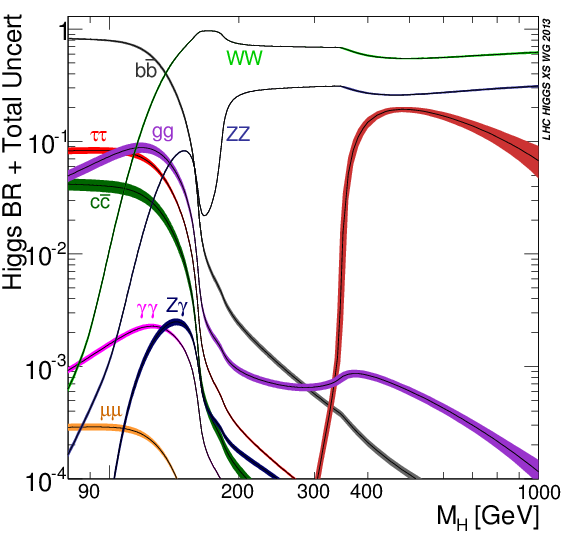
\includegraphics[width=3in]{images/Higgs_BR.png}
  \begin{tabular}{ |l|l| }
    \hline
    \multicolumn{2}{|c|}{Higgs Branching Ratios} \\
    \hline
    ${\rm b\bar{b}}$ & 0.57 \\
    WW & 0.22\\
    gg & 0.085 \\
    ${\rm \tau\tau}$ & 0.065 \\
    ZZ & 0.027 \\
    ${\rm c\bar{c}}$ & 0.027 \\
    ${\rm \gamma\gamma}$ & 0.0023 \\
    ${\rm Z}\gamma$ & 0.0016 \\
    ${\rm \mu^{+}\mu^{-}}$ & 0.00022 \\
    \hline
  \end{tabular} 
  \caption
{The graphic on the top left presents the SM Higgs branching fractions as functions of mass while the table on the bottom right displays the branching fractions for a 125 GeV SM Higgs \cite{crossbranchplots}.}
  \label{fig:hbranch}
\end{figure}

The muon has the lowest mass -- excluding the photon and gluon -- of the particles in Figure ~\ref{fig:hbranch} and consequently H$\rightarrow \mu^{+}\mu^{-}$ has the lowest branching fraction in the set. \footnote{The Higgs also couples to the electron and the first generation quarks but the masses are so light that CMS does not expect to see the SM Higgs in those modes.} The gluons and photons are massless and do not couple to the Higgs at leading order. These massless vector bosons interact with the Higgs through a loop of top quarks. The extremely heavy mass of the top quark, about 173 GeV, balances the fact that the loop production is a higher order mechanism.  
\begin{figure}[h!]
  \centering
  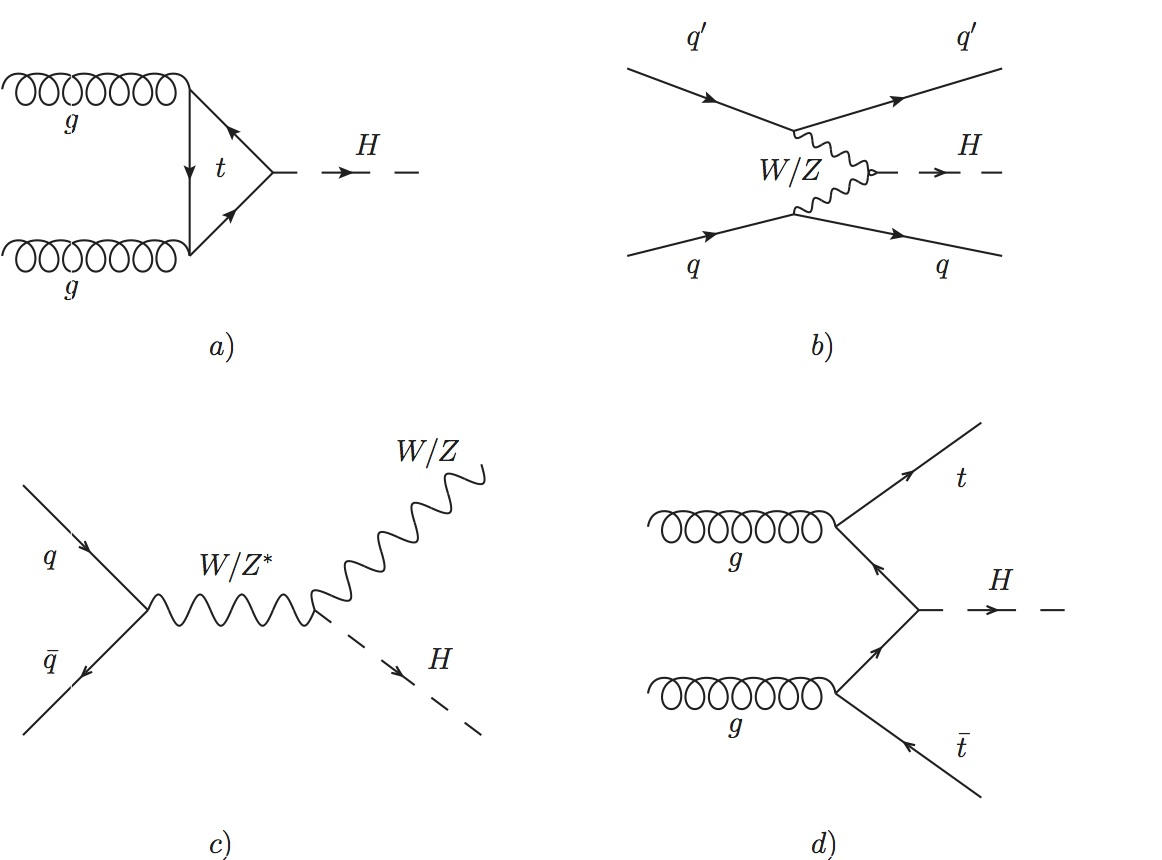
\includegraphics[width=4in]{images/higgs_production_modes.png}
  \caption
   {The SM production modes with the highest cross sections. a) Gluon Gluon Fusion (GF) b) Vector Boson Fusion (VBF) c) Associated Production with a Vector Boson (VH) d) ${\rm t\bar{t}}$H}
  \label{fig:hfeynprod}
\end{figure}

The Higgs to massless vector boson coupling via the top loop is seen in the GF Feynman diagram in Figure ~\ref{fig:hfeynprod}. At ${\rm M_{h} = 125}$ GeV, ${\rm \sqrt{s} =}$ 13 TeV, the GF channel comprises 87\% of the total Higgs production cross section, VBF 7\%, VH 4\%, and ${\rm t\bar{t}}$H 1\% \cite{crossbranchplots}. Besides ${\rm t\bar{t}}$H, the process q + $\bar{q} \rightarrow$ H isn't considered due to its low cross section. The low masses of the other quarks suppress the process. 

Quark gluon (qg) scattering is a major background for the Higgs to two jets decays since the process closely resembles GF in this mode.   

\begin{figure}[h!]
  \centering
  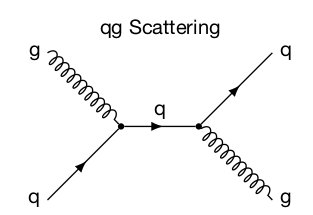
\includegraphics[width=2in]{images/qg_scattering.png}
  \caption
   {Quark gluon scattering creates many two jet events. This background looks very similar to GF when the Higgs decays to two jets. The colliding protons are made of quarks and gluons so this process is extremely common.}
  \label{fig:feynqg}
\end{figure}


\include{tex/search}
%\chapter{RESULTS} \label{results}

\section{Fusce Eget Tempus Lectus, }

%\hline
\begin{algorithm}  {Euclid’s algorithm}
%\hline %
\singlespacing

\begin{algorithmic}[1]
%\caption{Euclid’s algorithm}\label{alg:euclid}
\Procedure{Euclid}{$a,b$}\Comment{The g.c.d. of a and b}
\State $r\gets a\bmod b$
\While{$r\not=0$}\Comment{We have the answer if r is 0}
\State $a\gets b$
\State $b\gets r$
\State $r\gets a\bmod b$
\EndWhile\label{euclidendwhile}
\State \textbf{return} $b$\Comment{The gcd is b}
\EndProcedure
%\hline
\end{algorithmic}
\end{algorithm}









\proposition{The Upsilon Function}

(1) If $\beta>0$ and $\alpha\neq0$, then for all $n\geq-1$,

$$I_{n}(c;\alpha; \beta; \delta) = - \frac{e^{\alpha c}}{\alpha} \sum_{i=0}^{n}(\frac{\beta}{\alpha})^{n-i} Hh_{i}(\beta c -\delta)$$

$$+ (\frac{\beta}{\alpha})^{n+1} \frac{\sqrt{2 \pi}}{\beta} e^{\frac{\alpha \delta}{\beta}+\frac{\alpha^{2}}{2\beta^{2}}} \phi(-\beta c + \delta + \frac{\alpha}{\beta})$$
(2) If $\beta<0$ and $\alpha<0$, then for all $x \geq -1$

$$I_{n}(c;\alpha; \beta; \delta) = - \frac{e^{\alpha c}}{\alpha} \sum_{i=0}^{n}(\frac{\beta}{\alpha})^{n-i} Hh_{i}(\beta c -\delta)$$

$$- (\frac{\beta}{\alpha})^{n+1} \frac{\sqrt{2 \pi}}{\beta} e^{\frac{\alpha \delta}{\beta}+\frac{\alpha^{2}}{2\beta^{2}}} \phi(\beta c - \delta - \frac{\alpha}{\beta})$$

\begin{proof}{Case 1.}

$\beta>0$ and $\alpha\neq0$. Since, for any constant $\alpha$ and $n \geq 0$, $e^{\alpha x} Hh_{n}(\beta x - \delta) \rightarrow 0$ as $x \rightarrow \infty$ thanks to (B4), integration by parts leads to

$$I_{n}=-\frac{1}{\alpha}Hh(\beta c -\delta) e^{\alpha c} + \frac{\beta}{\alpha}\int_{c}^{\infty} e^{\alpha x} Hh_{n-1}(\beta c - \delta)dx$$

In other words, we have a recursion, for $n \geq 0$, $I_{n}=-(e^{\alpha c}{\alpha})Hh_{n}(\beta c - \delta) + (\frac{\beta}{\alpha})I_{n-1}$ with

$$I_{-1}=\sqrt{2 \pi} \int_{c}{\infty}e^{\alpha x}\varphi(-\beta x +\delta)dx$$

$$=\frac{\sqrt{2 \pi}}{\beta} e^{\frac{\alpha \delta}{\beta}+\frac{\alpha^{2}}{2 \beta^{2}}}\phi(-\beta c + \delta +\frac{\alpha}{\beta})$$

Solving it yields, for $n \geq -1$,

$$I_{n}=-\frac{e^{\alpha c}}{\alpha}\sum_{i=0}^{n}(\frac{\beta}{\alpha})^{i}Hh_{n-i}(\beta c+\delta) + (\frac{\beta}{\alpha})^{n+1}I_{-1}$$

$$=-\frac{e^{\alpha c}}{\alpha}\sum_{i=0}^{n}(\frac{\beta}{\alpha})^{n-i} Hh_{i}(\beta c+\delta)$$

$$+ (\frac{\beta}{\alpha})^{n+1}\frac{\sqrt{2 \pi}}{\beta} e^{\frac{\alpha \delta}{\beta}+\frac{\alpha^{2}}{2 \beta^{2}}}\phi(-\beta c + \delta +\frac{\alpha}{\beta})$$

where the sum over an empty set is defined to be zero.
\end{proof}

\begin{proof}{Case2.} $\beta<0$ and $\alpha<0$. In this case, we must also have, for $n \geq 0$ and any constant $\alpha<0, e^{\alpha x}Hh_{n}(\beta x -\delta) \rightarrow 0$ as

$x \rightarrow \infty$, thanks to (B5). Using integration by parts, we again have the same recursion, for $n \geq 0, I_{n}=-(e^{\alpha c}/\alpha)Hh_{n}(\beta c - \delta)+(\beta / \alpha)I_{n-1}$, but with a different initial condition

$$I_{-1}=\sqrt{2 \pi}\int_{c}^{\infty}e^{\alpha x}\varphi(-\beta x + \delta)dx$$

$$=-\frac{\sqrt{2 \pi}}{\beta} exp\{\frac{\alpha \delta}{\beta}+\frac{\alpha^{2}}{2 \beta^{2}}\}\phi(\beta c - \delta -\frac{\alpha}{\beta})$$

Solving it yields (B8), for $n \geq -1$.

\end{proof}

Finally, we sum the double exponential and the normal random variables

Proposition B.3.

Suppose $\{\xi_{1},\xi_{2},...\}$ is a sequence of i.i.d. exponential random variables with rate $\eta>0$, and Z is a normal variable with distribution $N(0,\sigma^{2})$. Then for every $ n \geq 1$, we have: (1) The density functions are given by:

$$f_{Z+\sum_{i=1}^{n}\xi_{i}}(t)=(\sigma\eta)^{n}\frac{e^{(\sigma\eta)^{2}/2}}{\sigma\sqrt{2\pi}}e^{-t\eta}Hh_{n-1}(-\frac{t}{\sigma}+\sigma\eta)$$

$$f_{Z-\sum_{i=1}^{n}\xi_{i}}(t)=(\sigma\eta)^{n}\frac{e^{(\sigma\eta)^{2}/2}}{\sigma\sqrt{2\pi}}e^{-t\eta}Hh_{n-1}(\frac{t}{\sigma}+\sigma\eta)$$
(2) The tail probabilities are given by

$$P(Z+\sum_{i=1}^{n}\xi_{i}\geq x) = (\sigma\eta)^{n}\frac{e^{(\sigma\eta)^{2}/2}}{\sigma\sqrt{2\pi}}e^{-t\eta}I_{n-1}(x;-\eta,-\frac{1}{\sigma},-\sigma\eta)$$

$$P(Z-\sum_{i=1}^{n}\xi_{i}\geq x) = (\sigma\eta)^{n}\frac{e^{(\sigma\eta)^{2}/2}}{\sigma\sqrt{2\pi}}e^{-t\eta}I_{n-1}(x;\eta,\frac{1}{\sigma},-\sigma\eta)$$

Proof. Case 1. The densities of $Z+\sum_{i=1}^{n}\xi_{i}$, and $Z-\sum_{i=1}^{n}\xi_{i}$. We have

$$f_{Z+\sum_{i=1}^{n}\xi_{i}}(t)=\int_{-\infty}^{\infty}f_{\sum_{i=1}^{n}\xi_{i}}(t-x)f_{Z}(x)dx$$

$$=e^{-t\eta}(\eta^{n})\int_{-\infty}{t}\frac{e^{x\eta}(t-x)^{n-1}}{(n-1)!}\frac{1}{\sigma\sqrt{2\pi}}e^{-x^{2}/(2\sigma^{2})}dx$$

$$=e^{-t\eta}(\eta^{n})e^{(\sigma\eta)^{2}/(2)}\int_{-\infty}{t}\frac{(t-x)^{n-1}}{(n-1)!}\frac{1}{\sigma\sqrt{2\pi}}e^{-(x-\sigma^{2}\eta)^{2}/(2\sigma^{2})}dx$$

Letting $y=(x-\sigma^{2}\eta)/\sigma$ yields

$$f_{Z+\sum_{i=1}^{n}\xi_{i}}(t)=e^{-t\eta}(\eta^{n})e^{(\sigma\eta)^{2}/(2)}\sigma^{n-1}$$

$$\times\int_{-\infty}^{t/\sigma-\sigma\eta}\frac{(t/\sigma - y -\sigma\eta)^{n-1}}{(n-1)!}\frac{1}{\sqrt{2\pi}}e^{-y^{2}/2}dy$$

$$=\frac{e^{(\sigma\eta)^{2}/2}}{\sqrt{2\pi}}(\sigma^{n-1}\eta^{n})e^{-t\eta}Hh_{n-1}(-t/\sigma + \sigma\eta)$$

because $(1/(n-1)!)\int_{-\infty}{a}(a-y)^{n-1}e^{-y^{2}/2}dy=Hh_{n-1}(a)$. The derivation of $f_{Z+\sum_{i=1}^{n}\xi_{i}}(t)$ is similar.

Case 2. $P(Z+\sum_{i=1}^{n}\xi_{i}\geq x)$ and $P(Z-\sum_{i=1}^{n}\xi_{i}\geq x)$. From (B9), it is clear that

$$P(Z+\sum_{i=1}^{n}\xi_{i}\geq x)=\frac{(\sigma\eta)^{n}e^{(\sigma\eta)^{2}/2}}{\sigma\sqrt{2\pi}}\int_{x}^{\infty}e^{(-i\eta)}Hh_{n-1}(-\frac{t}{\sigma}+\sigma\eta)dt$$

$$=\frac{(\sigma\eta)^{n}e^{(\sigma\eta)^{2}/2}}{\sigma\sqrt{2\pi}}I_{n-1}(x;-\eta,-\frac{1}{\sigma},-\sigma\eta)dt$$

by (B6). We can compute
$P(Z-\sum_{i=1}^{n}\xi_{i}\geq x)$ similarly.

\theorem{Theorem} With $\pi_{n}:= P(N(t)=n)=e^{-\lambda T}(\lambda T)^{n}/n!$ and $I_{n}$ in Proposition \ref{first}.
, we have

$$P(Z(T)\geq a)=\frac{e^{(\sigma \eta_{1})^{2} T/2}}{\sigma \sqrt{2 \pi T}} \sum_{n=1}^{\infty} \pi_{n} \sum_{k=1}^{n} P_{n,k}(\sigma\sqrt{T}\eta_{1})^{k}\times I_{k-1}(a-\mu T; -\eta_{1},-\frac{1}{\sigma\sqrt{T}},-\sigma\eta_{1}\sqrt{T})$$

$$+\frac{e^{(\sigma\eta_{2})^{2}T/2}}{\sigma\sqrt{2\pi T}}\sum_{n=1}^{\infty}\pi_{n}\sum_{k=1}^{n}Q_{n,k}(\sigma\sqrt{T}\eta_{2})^{k}$$

$$\times I_{k-1}(a-\mu T; \eta_{2},\frac{1}{\sigma\sqrt{T}},-\sigma\eta_{2}\sqrt{T})$$

$$+\pi_{0}\phi(-\frac{a-\mu T}{\sigma\sqrt{T}})$$

Proof by the decomposition (B2)

$$P(Z(T) \geq a)= \sum_{n=0}^{\infty}\pi_{n} P(\mu T +\sigma\sqrt{T} Z + \sum_{j=1}^{n}Y_{j} \geq a)$$

$$=\pi_{0}P(\mu T +\sigma\sqrt{T} Z  \geq a)$$

$$+\sum_{n=1}^{\infty}\pi_{n}\sum_{k=1}^{n}P_{n,k} P(\mu T +\sigma\sqrt{T} Z + \sum_{j=1}^{n}\xi_{j}^{+} \geq a)$$

$$+\sum_{n=1}^{\infty}\pi_{n}\sum_{k=1}^{n}Q_{n,k} P(\mu T +\sigma\sqrt{T} Z - \sum_{j=1}^{n}\xi_{j}^{-} \geq a)$$

The result now follows via (B11) and (B12) for $\eta_{1} > 1$ and $\eta_{2} >0$. 
%\chapter{SUMMARY AND CONCLUSIONS} \label{conclusion}

\section{Non Porttitor Tellus}

Aliquam molestie sed urna quis convallis. Aenean nibh eros, aliquam non eros in, tempus lacinia justo. In magna sapien, blandit a faucibus ac, scelerisque nec purus. Praesent fermentum felis nec massa interdum, vel dapibus mi luctus. Cras id fringilla mauris. Ut molestie eros mi, ut hendrerit nulla tempor et. Pellentesque tortor quam, mattis a scelerisque nec, euismod et odio. Mauris rhoncus metus sit amet risus mattis, eu mattis sem interdum.

\subsection{Nam Arcu Magna}
Semper vel lorem eu, venenatis ultrices est. Nam aliquet ut erat ac scelerisque. Maecenas ut molestie mi. Phasellus ipsum magna, sollicitudin eu ipsum quis, imperdiet cursus turpis. Etiam pretium enim a fermentum accumsan. Morbi vel vehicula enim.

\subsubsection{Ut pellentesque velit sede}
 Placerat cursus. Integer congue urna non massa dictum, a pellentesque arcu accumsan. Nulla posuere, elit accumsan eleifend elementum, ipsum massa tristique metus, in ornare neque nisl sed odio. Nullam eget elementum nisi. Duis a consectetur erat, sit amet malesuada sapien. Aliquam nec sapien et leo sagittis porttitor at ut lacus. Vivamus vulputate elit vitae libero condimentum dictum. Nulla facilisi. Quisque non nibh et massa ullamcorper iaculis.


%\include{tex/chapter6}  %These chapters are not included in the template
%\include{tex/chapter7}

%-----------------------------------------------------------------------%

% Use the appropriate file depending upon the number of appendices you have


%% The Editorial Office Requirements for the Table of Contents cause a significant problem
%in Latex if there is only one Appendix. The Appendix is no longer labeled "A" in the TOC
%but has the word "APPENDIX" placed in front of the title of the Appendix. This can be done
%without issue IF nothing needs to be numbered by LaTeX in the Appendix. Unfortunately, most of the time
%something needs to be numbered in that single Appendix. For this reason we have included the IFTHENELSE switch
%found in this document and at the beginning of AppendixA. We assume that if you have any appendices, that you have more than one. However, you DO only have one appendix DO NOT USE THIS FILE!!!!!!!!!!!!!!!!!!!!!!!
%
% OneSingleAppendix.tex has all the settings needed to adjust for a single appendix
% you will have a major problem with your TOC if you use this file with a single appendix!!!!!

%
% Comment (or delete) all of the \input{AppendixB} commands except those you are using.
%Then open the AppendixA.tex file and continue there.

%you can add/substract individual appendices through by using the /include{appendix'X'}
% and creating/deleting the appropriate files
\appendix %
%\clearpage%

\addtocontents{toc}{\protect\addvspace{10pt}\noindent{APPENDIX} \protect\hfill\par}{}


% % % % % % % If you have a single appendix, you should be using appendix1.tex
% % % % % % % NOT this file

\chapter{THIS IS THE FIRST APPENDIX}

Lorem ipsum dolor sit amet, consectetuer adipiscing elit. Maecenas
eget magna. Aenean et lorem. Ut dignissim neque at nisi. In hac
habitasse platea dictumst. In porta ornare eros. Nunc eu ante. In
non est vehicula tellus cursus suscipit. Proin sed libero. Sed risus
enim, eleifend in, pellentesque ac, nonummy quis, nulla. Phasellus
imperdiet libero nec massa. Ut sapien libero, adipiscing eu,
volutpat porttitor, ultricies eget, nisi. Sed odio. Suspendisse
potenti. Duis dolor augue, viverra id, porta in, dignissim id, nisl.
Vivamus blandit cursus eros. Maecenas sit amet urna sit amet orci
nonummy pharetra.

Praesent cursus nibh et mauris. In aliquam felis sit amet ligula.
Nulla faucibus nisl eget nisl. Aliquam tincidunt. Mauris eget elit
sed massa luctus posuere. Pellentesque suscipit. In odio urna,
semper ut, convallis ut, porta et, nibh. Nulla sodales metus nec
velit posuere gravida. Cras tristique. Etiam urna risus, accumsan
ut, placerat sed, iaculis id, est.

Nullam mi. Pellentesque habitant morbi tristique senectus et netus
et malesuada fames ac turpis egestas. Duis vitae metus in massa
hendrerit rhoncus. Fusce tortor justo, laoreet eu, facilisis at,
gravida et, felis. Donec imperdiet mollis erat. Integer tempus nulla
ac lorem. Fusce porttitor. Aenean quis arcu. Morbi consectetuer, leo
eu mollis elementum, urna massa malesuada risus, euismod tempor
lorem elit ut mauris. Cras elit orci, facilisis ac, mattis iaculis,
cursus ac, augue. Donec eget nisl. Pellentesque fermentum sodales
nibh. Vivamus non risus. Donec est libero, tincidunt sit amet,
pretium vitae, blandit sed, tellus. Nunc diam risus, interdum sed,
laoreet quis, varius ac, turpis. In et purus eget nibh vehicula
rhoncus. Aenean et neque. Praesent nisl nisi, tempus quis, nonummy
ac, auctor a, neque. Suspendisse et metus. Suspendisse non metus eu
mauris auctor sagittis.
 %
\chapter{AN EXAMPLE OF A HALF TITLE PAGE}%
\label{appendixB}

\clearpage %remove this command if your appendix doesn't start with a landscaped page!!!!!
\thispagestyle{plain}
\begin{landscape}
\begin{figure}

  \begin{center}
    \includegraphics[width=6in]{images/LaTeX2e_logo.eps}
    \caption{\LaTeX 2\ensuremath{\epsilon.} logo}\label{biglogo}
  \end{center}
\end{figure}
\end{landscape}


This is how a section should look if the first page is a landscape page.
Lorem ipsum dolor sit amet, consectetuer adipiscing elit. Ut sit
amet nulla. Integer mauris turpis, dapibus ac, auctor non, vehicula
sit amet, magna. Suspendisse eu tellus. Etiam porta. Donec magna.
Donec ut dui. In hac habitasse platea dictumst. Nullam suscipit, mi
at adipiscing commodo, lorem erat scelerisque erat, non pulvinar leo
mi eu metus. Phasellus id felis. Sed quam purus, molestie quis,
ultrices nec, dictum at, magna. Proin viverra viverra ante.

Maecenas sagittis magna quis ligula. Duis vestibulum mi a felis.
Aenean accumsan mattis massa. Nullam lacus sem, consectetuer non,
condimentum sit amet, pharetra ac, odio. Morbi nisi magna, tincidunt
sed, placerat nec, tincidunt id, lectus. Donec ac dui non mauris
vulputate aliquam. Nullam scelerisque congue pede. Integer ipsum.
Vestibulum auctor. Suspendisse eget leo id libero cursus dictum. Sed
malesuada. Aliquam imperdiet. Donec dui metus, porta eu, aliquet
vel, vulputate vitae, lacus.

Nulla quis purus id turpis luctus feugiat. Fusce feugiat. Proin
felis. Morbi elit est, fermentum in, tincidunt vitae, convallis vel,
orci. Vestibulum justo. Suspendisse non nisl. Pellentesque pretium
adipiscing elit. Phasellus fermentum consequat augue. Sed pede nisl,
fermentum vel, vulputate id, sollicitudin sed, ligula. Cras
suscipit, quam et euismod sagittis, nisl felis gravida felis, quis
pulvinar purus est vel pede. Suspendisse mattis est ac nunc.
Curabitur rutrum, turpis sit amet commodo tempus, metus lorem
commodo lectus, eget fringilla justo nisi et purus. Ut quam sapien,
vehicula quis, rhoncus non, sagittis nec, risus.

Donec eget augue ac lacus adipiscing porta. Maecenas pede. Vivamus
molestie. Duis condimentum ligula auctor pede. Nullam ullamcorper
rhoncus erat. Ut ornare interdum urna. Suspendisse potenti.
Curabitur mattis mauris nec risus. Aenean iaculis turpis eu tortor.
Donec nec ante non mauris pellentesque fringilla.

Phasellus vitae dui id orci sodales cursus. Curabitur sed nulla quis
mauris tincidunt iaculis. Vivamus semper semper orci. Phasellus
suscipit ante vitae leo. Sed arcu ipsum, condimentum id, luctus in,
sodales eu, magna. In dictum, arcu quis pharetra vestibulum, ante
enim placerat lacus, vitae placerat est leo vitae elit. Pellentesque
bibendum enim vulputate eros. Nunc laoreet. Pellentesque habitant
morbi tristique senectus et netus et malesuada fames ac turpis
egestas. Praesent purus odio, euismod sit amet, aliquam a, volutpat
in, augue. Phasellus id massa. Suspendisse suscipit ligula pharetra
dolor. Pellentesque vel pede.

Aliquam pharetra est sit amet magna. Aliquam varius. Donec eu lectus
et nisl iaculis porttitor. Morbi mattis, mauris sed luctus
hendrerit, nulla velit molestie dolor, ac volutpat urna augue vel
quam. Maecenas pellentesque libero et massa. Integer vestibulum,
lacus at mattis euismod, nisl arcu commodo lectus, ut euismod dolor
ligula sit amet libero. Nam in ligula sit amet ante eleifend
aliquet. Phasellus feugiat erat at nulla. Proin in lectus. Proin
laoreet leo laoreet leo congue lacinia. Quisque non diam sit amet
enim ultrices commodo. Praesent fermentum lectus sed ligula. Integer
pulvinar accumsan pede. Quisque molestie ligula eget odio.
Vestibulum ante ipsum primis in faucibus orci luctus et ultrices
posuere cubilia Curae;
 %
\chapter{DERIVATION OF THE $\Upsilon$ FUNCTION}%
\label{appendixC}

%\clearpage %remove this command if your appendix doesn't start with a landscaped page!!!!!
%\thispagestyle{plain}
%\begin{landscape}
%\begin{figure}

 % \begin{center}
  %  \includegraphics[width=6in]{LaTeX2e_logo.eps}
   % \caption{\LaTeX 2\ensuremath{\epsilon.} logo}\label{biglogo}
  %\end{center}
%\end{figure}
%\end{landscape}

%%%%%%%%%%%%%%%%%%%%%%%%%%%%%%%%%%%%%%%%%%%%%%%%%%%%%%%%%%%%%%%%%%%%%%%%%%%%%%%%%%%%%%%%%%%%%%%%%%


%ADD LABEL

%%%%%%%%%%%%%%%%%%%%%%%%%%%%%%%%%%%%%%%%%%%%%%%%%%%%%%%%%%%%%%%%%%%%%%%%%%%%%%%%%%%%%%%%%%%%%%%%%%

\proposition{The Upsilon Function}

(1) If $\beta>0$ and $\alpha\neq0$, then for all $n\geq-1$,

$$I_{n}(c;\alpha; \beta; \delta) = - \frac{e^{\alpha c}}{\alpha} \sum_{i=0}^{n}(\frac{\beta}{\alpha})^{n-i} Hh_{i}(\beta c -\delta)$$

$$+ (\frac{\beta}{\alpha})^{n+1} \frac{\sqrt{2 \pi}}{\beta} e^{\frac{\alpha \delta}{\beta}+\frac{\alpha^{2}}{2\beta^{2}}} \phi(-\beta c + \delta + \frac{\alpha}{\beta})$$
(2) If $\beta<0$ and $\alpha<0$, then for all $x \geq -1$

$$I_{n}(c;\alpha; \beta; \delta) = - \frac{e^{\alpha c}}{\alpha} \sum_{i=0}^{n}(\frac{\beta}{\alpha})^{n-i} Hh_{i}(\beta c -\delta)$$

$$- (\frac{\beta}{\alpha})^{n+1} \frac{\sqrt{2 \pi}}{\beta} e^{\frac{\alpha \delta}{\beta}+\frac{\alpha^{2}}{2\beta^{2}}} \phi(\beta c - \delta - \frac{\alpha}{\beta})$$

\begin{proof}{Case 1.}

$\beta>0$ and $\alpha\neq0$. Since, for any constant $\alpha$ and $n \geq 0$, $e^{\alpha x} Hh_{n}(\beta x - \delta) \rightarrow 0$ as $x \rightarrow \infty$ thanks to (B4), integration by parts leads to

$$I_{n}=-\frac{1}{\alpha}Hh(\beta c -\delta) e^{\alpha c} + \frac{\beta}{\alpha}\int_{c}^{\infty} e^{\alpha x} Hh_{n-1}(\beta c - \delta)dx$$

In other words, we have a recursion, for $n \geq 0$, $I_{n}=-(e^{\alpha c}{\alpha})Hh_{n}(\beta c - \delta) + (\frac{\beta}{\alpha})I_{n-1}$ with

$$I_{-1}=\sqrt{2 \pi} \int_{c}{\infty}e^{\alpha x}\varphi(-\beta x +\delta)dx$$

$$=\frac{\sqrt{2 \pi}}{\beta} e^{\frac{\alpha \delta}{\beta}+\frac{\alpha^{2}}{2 \beta^{2}}}\phi(-\beta c + \delta +\frac{\alpha}{\beta})$$

Solving it yields, for $n \geq -1$,

$$I_{n}=-\frac{e^{\alpha c}}{\alpha}\sum_{i=0}^{n}(\frac{\beta}{\alpha})^{i}Hh_{n-i}(\beta c+\delta) + (\frac{\beta}{\alpha})^{n+1}I_{-1}$$

$$=-\frac{e^{\alpha c}}{\alpha}\sum_{i=0}^{n}(\frac{\beta}{\alpha})^{n-i} Hh_{i}(\beta c+\delta)$$

$$+ (\frac{\beta}{\alpha})^{n+1}\frac{\sqrt{2 \pi}}{\beta} e^{\frac{\alpha \delta}{\beta}+\frac{\alpha^{2}}{2 \beta^{2}}}\phi(-\beta c + \delta +\frac{\alpha}{\beta})$$

where the sum over an empty set is defined to be zero.
\end{proof}

Case2. $\beta<0$ and $\alpha<0$. In this case, we must also have, for $n \geq 0$ and any constant $\alpha<0, e^{\alpha x}Hh_{n}(\beta x -\delta) \rightarrow 0$ as

$x \rightarrow \infty$, thanks to (B5). Using integration by parts, we again have the same recursion, for $n \geq 0, I_{n}=-(e^{\alpha c}/\alpha)Hh_{n}(\beta c - \delta)+(\beta / \alpha)I_{n-1}$, but with a different initial condition

$$I_{-1}=\sqrt{2 \pi}\int_{c}^{\infty}e^{\alpha x}\varphi(-\beta x + \delta)dx$$

$$=-\frac{\sqrt{2 \pi}}{\beta} exp\{\frac{\alpha \delta}{\beta}+\frac{\alpha^{2}}{2 \beta^{2}}\}\phi(\beta c - \delta -\frac{\alpha}{\beta})$$

Solving it yields (B8), for $n \geq -1$.

Finally, we sum the double exponential and the normal random variables

Proposition B.3.

Suppose $\{\xi_{1},\xi_{2},...\}$ is a sequence of i.i.d. exponential random variables with rate $\eta>0$, and Z is a normal variable with distribution $N(0,\sigma^{2})$. Then for every $ n \geq 1$, we have: (1) The density functions are given by:

$$f_{Z+\sum_{i=1}^{n}\xi_{i}}(t)=(\sigma\eta)^{n}\frac{e^{(\sigma\eta)^{2}/2}}{\sigma\sqrt{2\pi}}e^{-t\eta}Hh_{n-1}(-\frac{t}{\sigma}+\sigma\eta)$$

$$f_{Z-\sum_{i=1}^{n}\xi_{i}}(t)=(\sigma\eta)^{n}\frac{e^{(\sigma\eta)^{2}/2}}{\sigma\sqrt{2\pi}}e^{-t\eta}Hh_{n-1}(\frac{t}{\sigma}+\sigma\eta)$$
(2) The tail probabilities are given by

$$P(Z+\sum_{i=1}^{n}\xi_{i}\geq x) = (\sigma\eta)^{n}\frac{e^{(\sigma\eta)^{2}/2}}{\sigma\sqrt{2\pi}}e^{-t\eta}I_{n-1}(x;-\eta,-\frac{1}{\sigma},-\sigma\eta)$$

$$P(Z-\sum_{i=1}^{n}\xi_{i}\geq x) = (\sigma\eta)^{n}\frac{e^{(\sigma\eta)^{2}/2}}{\sigma\sqrt{2\pi}}e^{-t\eta}I_{n-1}(x;\eta,\frac{1}{\sigma},-\sigma\eta)$$

Proof. Case 1. The densities of $Z+\sum_{i=1}^{n}\xi_{i}$, and $Z-\sum_{i=1}^{n}\xi_{i}$. We have

$$f_{Z+\sum_{i=1}^{n}\xi_{i}}(t)=\int_{-\infty}^{\infty}f_{\sum_{i=1}^{n}\xi_{i}}(t-x)f_{Z}(x)dx$$

$$=e^{-t\eta}(\eta^{n})\int_{-\infty}{t}\frac{e^{x\eta}(t-x)^{n-1}}{(n-1)!}\frac{1}{\sigma\sqrt{2\pi}}e^{-x^{2}/(2\sigma^{2})}dx$$

$$=e^{-t\eta}(\eta^{n})e^{(\sigma\eta)^{2}/(2)}\int_{-\infty}{t}\frac{(t-x)^{n-1}}{(n-1)!}\frac{1}{\sigma\sqrt{2\pi}}e^{-(x-\sigma^{2}\eta)^{2}/(2\sigma^{2})}dx$$

Letting $y=(x-\sigma^{2}\eta)/\sigma$ yields

$$f_{Z+\sum_{i=1}^{n}\xi_{i}}(t)=e^{-t\eta}(\eta^{n})e^{(\sigma\eta)^{2}/(2)}\sigma^{n-1}$$

$$\times\int_{-\infty}^{t/\sigma-\sigma\eta}\frac{(t/\sigma - y -\sigma\eta)^{n-1}}{(n-1)!}\frac{1}{\sqrt{2\pi}}e^{-y^{2}/2}dy$$

$$=\frac{e^{(\sigma\eta)^{2}/2}}{\sqrt{2\pi}}(\sigma^{n-1}\eta^{n})e^{-t\eta}Hh_{n-1}(-t/\sigma + \sigma\eta)$$

because $(1/(n-1)!)\int_{-\infty}{a}(a-y)^{n-1}e^{-y^{2}/2}dy=Hh_{n-1}(a)$. The derivation of $f_{Z+\sum_{i=1}^{n}\xi_{i}}(t)$ is similar.

Case 2. $P(Z+\sum_{i=1}^{n}\xi_{i}\geq x)$ and $P(Z-\sum_{i=1}^{n}\xi_{i}\geq x)$. From (B9), it is clear that

$$P(Z+\sum_{i=1}^{n}\xi_{i}\geq x)=\frac{(\sigma\eta)^{n}e^{(\sigma\eta)^{2}/2}}{\sigma\sqrt{2\pi}}\int_{x}^{\infty}e^{(-i\eta)}Hh_{n-1}(-\frac{t}{\sigma}+\sigma\eta)dt$$

$$=\frac{(\sigma\eta)^{n}e^{(\sigma\eta)^{2}/2}}{\sigma\sqrt{2\pi}}I_{n-1}(x;-\eta,-\frac{1}{\sigma},-\sigma\eta)dt$$

by (B6). We can compute
$P(Z-\sum_{i=1}^{n}\xi_{i}\geq x)$ similarly.

\theorem{Theorem} With $\pi_{n}:= P(N(t)=n)=e^{-\lambda T}(\lambda T)^{n}/n!$ and $I_{n}$ in Proposition \ref{first}.
, we have

$$P(Z(T)\geq a)=\frac{e^{(\sigma \eta_{1})^{2} T/2}}{\sigma \sqrt{2 \pi T}} \sum_{n=1}^{\infty} \pi_{n} \sum_{k=1}^{n} P_{n,k}(\sigma\sqrt{T}\eta_{1})^{k}\times I_{k-1}(a-\mu T; -\eta_{1},-\frac{1}{\sigma\sqrt{T}},-\sigma\eta_{1}\sqrt{T})$$

$$+\frac{e^{(\sigma\eta_{2})^{2}T/2}}{\sigma\sqrt{2\pi T}}\sum_{n=1}^{\infty}\pi_{n}\sum_{k=1}^{n}Q_{n,k}(\sigma\sqrt{T}\eta_{2})^{k}$$

$$\times I_{k-1}(a-\mu T; \eta_{2},\frac{1}{\sigma\sqrt{T}},-\sigma\eta_{2}\sqrt{T})$$

$$+\pi_{0}\phi(-\frac{a-\mu T}{\sigma\sqrt{T}})$$

Proof by the decomposition (B2)

$$P(Z(T) \geq a)= \sum_{n=0}^{\infty}\pi_{n} P(\mu T +\sigma\sqrt{T} Z + \sum_{j=1}^{n}Y_{j} \geq a)$$

$$=\pi_{0}P(\mu T +\sigma\sqrt{T} Z  \geq a)$$

$$+\sum_{n=1}^{\infty}\pi_{n}\sum_{k=1}^{n}P_{n,k} P(\mu T +\sigma\sqrt{T} Z + \sum_{j=1}^{n}\xi_{j}^{+} \geq a)$$

$$+\sum_{n=1}^{\infty}\pi_{n}\sum_{k=1}^{n}Q_{n,k} P(\mu T +\sigma\sqrt{T} Z - \sum_{j=1}^{n}\xi_{j}^{-} \geq a)$$

The result now follows via (B11) and (B12) for $\eta_{1} > 1$ and $\eta_{2} >0$.


 %
\chapter{DERIVATION OF THE $\Upsilon$ FUNCTION}%
\label{appendixB}

%\clearpage %remove this command if your appendix doesn't start with a landscaped page!!!!!
%\thispagestyle{plain}
%\begin{landscape}
%\begin{figure}

% \begin{center}
  %  \includegraphics[width=6in]{LaTeX2e_logo.eps}
   % \caption{\LaTeX 2\ensuremath{\epsilon.} logo}\label{biglogo}
  %\end{center}
%\end{figure}
%\end{landscape}

%%%%%%%%%%%%%%%%%%%%%%%%%%%%%%%%%%%%%%%%%%%%%%%%%%%%%%%%%%%%%%%%%%%%%%%%%%%%%%%%%%%%%%%%%%%%%%%%%%

%ADD LABEL

%%%%%%%%%%%%%%%%%%%%%%%%%%%%%%%%%%%%%%%%%%%%%%%%%%%%%%%%%%%%%%%%%%%%%%%%%%%%%%%%%%%%%%%%%%%%%%%%%%

We first decompose the sum of the double exponential random variables.

The memoryless property of exponential random variables yields $(\xi^{+}-\xi^{-}|\xi^{+}>\xi^{-})=^{d}\xi^{+}$ and $(\xi^{+}-\xi^{-}|\xi^{+}<\xi^{-})=^{d}-\xi^{-}$, thus leading to the conclusion that

\begin{equation*}
\xi^{+}-\xi^{-} =\left\{
\begin{array}{rl}
\xi^{+} & \text{with probability $\eta_{2}/(\eta_{1}+\eta_{2})$ }\\
-\xi^{-} & \text{with probability $\eta_{1}/(\eta_{1}+\eta_{2})$ }
\end{array}\right\}.
\end{equation*}

because the probabilities of the events $\xi^{+}>\xi^{-}$ and $\xi^{+}<\xi^{-}$ are $\eta_{2}/(\eta_{1}+\eta_{2})$ and $\eta_{1}/(\eta_{1}+\eta_{2})$, respectively. The following proposition extends (B.1.)

Proposition B.1. For every $n\geq1$, we have the following decomposition

\begin{equation*}
\sum_{i=1}^{n}Y_{i}=^{d}\left\{
\begin{array}{rl}
\sum_{i=1}^{k}\xi_{i}^{+} & \text{with probability $P_{n,k},k=1,2,...,n$ }\\
-\sum_{i=1}^{k}\xi_{i}^{-} & \text{with probability $Q_{n,k},k=1,2,...,n$ }
\end{array}\right\}.
\end{equation*}

where $P_{n,k}$ and $Q_{n,k}$ are given by

$$P_{n,k}=\sum_{i=k}^{n-1}\binom {n-k-1} {i-k}\binom {n} {i}(\frac{\eta_{1}}{\eta_{1}+\eta_{2}})^{i-k}(\frac{\eta_{2}}{\eta_{1}+\eta_{2}})^{n-i}p^{i}q^{n-i}$$

$$1\leq k\leq n-1$$

$$Q_{n,k}=\sum_{i=k}^{n-1}\binom {n-k-1} {i-k}\binom {n} {i}(\frac{\eta_{1}}{\eta_{1}+\eta_{2}})^{n-i}(\frac{\eta_{2}}{\eta_{1}+\eta_{2}})^{i-k}p^{n-i}q^{i}$$

$$1\leq k\leq n-1, P_{n,n}=p^{n},Q_{n,n}=q^{n}$$

and $\binom{0}{0}$ is defined to be one. Hence $\xi_{i}^{+}$ and $\xi_{i}^{-}$ are i.i.d. exponential random variables with rates $\eta_{1}$ and $\eta_{2}$, respectively.

As a key step in deriving closed-form solutions for call and put options, this proposition indicates that the sum of the i.i.d. double exponential random variable can be written, in distribution, as a randomly mixed gamma random variable. To prove Proposition B.1, the following lemma is needed.

Lemma B.1.

$$\sum_{i=1}^{n}\xi_{i}^{+}-\sum_{i=1}^{n}\xi_{i}^{-}$$

\begin{equation*}
=^{d}\left\{
\begin{array}{rl}
\sum_{i=1}^{k}\xi_{i} & \text{with probability $\binom {n-k+m-1} {m-1}(\frac{\eta_{1}}{\eta_{1}+\eta_{2}})^{n-k}(\frac{\eta_{2}}{\eta_{1}+\eta_{2}})^{m}, k=1,...,n$ }\\
-\sum_{i=1}^{l}\xi_{i} & \text{with probability $\binom {n-l+m-1} {n-1}(\frac{\eta_{1}}{\eta_{1}+\eta_{2}})^{n}(\frac{\eta_{2}}{\eta_{1}+\eta_{2}})^{m-l}, l=1,...,m$ }
\end{array}\right\}.
\end{equation*}

We prove it by introducing the random variables $A(n,m) = \sum_{i=1}^{n}\xi_{i}-sum_{j=1}^{m}\tilde{\xi}_{j}$ Then

\begin{equation*}
A(n,m) =^{d}\left\{
\begin{array}{rl}
A(n-1,m-1)+\xi^{+} & \text{with probability $\eta_{2}/(\eta_{1}+\eta_{2})$ }\\
A(n-1,m-1)-\xi^{-} & \text{with probability $\eta_{1}/(\eta_{1}+\eta_{2})$ }
\end{array}\right\}.
\end{equation*}

\begin{equation*}
 =^{d}\left\{
\begin{array}{rl}
A(n,m-1) & \text{with probability $\eta_{2}/(\eta_{1}+\eta_{2})$ }\\
A(n-1,m) & \text{with probability $\eta_{1}/(\eta_{1}+\eta_{2})$ }
\end{array}\right\}.
\end{equation*}

via B.1.. Now suppose horizontal axis that are representing the number of $\{\zeta_{i}^{+}\}$ and vertical axis representing the number of $\{\zeta_{i}^{-}\}$. Suppose we have a random walk on the integer lattice points. Starting from any point $(n,m),n,m \geq 1$, the random walk goes either one step to the left with probability $\eta_{1}/(\eta_{1}+\eta_{2})$ or one step down with probability $\eta_{2}/(\eta_{1}+\eta_{2})$, and the random walks stops once it reaches the horizontal or vertical axis. For any path from (n,m) to (k,0) , $1 \geq k \geq n$, it must reach (k,1) first before it makes a final move to (k,0). Furthermore, all the paths going from (n,m) to (k,1) must have exactly n-k lefts and m-1 downs, whence the total number of such paths is $\binom {n-k+m-1}{m-1}$. Similarly the total number of paths from (n,m) to (0,l) , $1 \geq l \geq m$, is $\binom {n-l+m-1}{n-1}$. Thus

\begin{equation*}
A(n,m)=^{d}\left\{
\begin{array}{rl}
\sum_{i=1}^{k}\xi_{i} & \text{with probability $\binom {n-k+m-1} {m-1}(\frac{\eta_{1}}{\eta_{1}+\eta_{2}})^{n-k}(\frac{\eta_{2}}{\eta_{1}+\eta_{2}})^{m}, k=1,...,n$ }\\
-\sum_{i=1}^{l}\xi_{i} & \text{with probability $\binom {n-l+m-1} {n-1}(\frac{\eta_{1}}{\eta_{1}+\eta_{2}})^{n}(\frac{\eta_{2}}{\eta_{1}+\eta_{2}})^{m-l}, l=1,...,m$ }
\end{array}\right\}.
\end{equation*}

and the lemma is proven.

Now, let's prove the proposition B.1. By the same analogy used in Lemma B.1 to compute probability $P_{n,m},1\geq k \geq n$, the probability weight assigned to $\sum_{i=1}^{k}\xi_{i}^{+}$ when we decompose $\sum_{i=1}^{k}Y_{i}$, it is equivalent to consider the probability of the random walk ever reach (k,0) starting from the point (i,n-i) being $\binom {n}{i}p^{i}q^{n-i}$. Note that the point (k,0) can only be reached from point (i,n-i) such that $k \geq i \geq n-1$, because the random walk can only go left or down, and stops once it reaches the horizontal axis. Therefore, for $1 \geq k \geq n-1$, (B3) leads to

$$P_{n,k}=\sum_{i=k}{n-1}P(going from (i,n-i) to (k,0)). P(starting from (i,n-i))$$

$$=\sum_{i=k}^{n-1}\binom {i+(n-i)-k-1} {(n-i)-1}\binom {n} {i}(\frac{\eta_{1}}{\eta_{1}+\eta_{2}})^{i-k}(\frac{\eta_{2}}{\eta_{1}+\eta_{2}})^{n-i}p^{i}q^{n-i}$$

$$=\sum_{i=k}^{n-1}\binom {n-k-1} {n-i-1}\binom {n} {i}(\frac{\eta_{1}}{\eta_{1}+\eta_{2}})^{i-k}(\frac{\eta_{2}}{\eta_{1}+\eta_{2}})^{n-i}p^{i}q^{n-i}$$

$$=\sum_{i=k}^{n-1}\binom {n-k-1} {i-k}\binom {n} {i}(\frac{\eta_{1}}{\eta_{1}+\eta_{2}})^{i-k}(\frac{\eta_{2}}{\eta_{1}+\eta_{2}})^{n-i}p^{i}q^{n-i}$$

Of course $P_{n,n}=p^{n}$. Similarly, we can compute $Q_{n,k}$:

$$Q_{n,k}=\sum_{i=k}{n-1}P(going from (n-i,i) to (0,k)). P(starting from (n-i,i))$$

$$=\sum_{i=k}^{n-1}\binom {i+(n-i)-k-1} {(n-i)-1}\binom {n} {n-i}(\frac{\eta_{1}}{\eta_{1}+\eta_{2}})^{n-i}(\frac{\eta_{2}}{\eta_{1}+\eta_{2}})^{i-k}p^{n-i}q^{i}$$

$$=\sum_{i=k}^{n-1}\binom {n-k-1} {i-k}\binom {n} {i}(\frac{\eta_{1}}{\eta_{1}+\eta_{2}})^{n-i}(\frac{\eta_{2}}{\eta_{1}+\eta_{2}})^{i-k}p^{n-i}q^{i}$$

with $Q_{n,n}=q^{n}$. Incidentally, we have also got $\sum{k=1}{n}(P_{n,k}+Q_{n,k})=1$

B.2. Let's develop now the results on Hh functions.
First of all, note that $Hh_{n}(x)\rightarrow 0$, as $x \rightarrow \infty$, for $n \geq -1$; and $Hh_{n}(x) \rightarrow \infty$, as $x \rightarrow -\infty$, for $n \geq -1$; and $Hh_{0}(x)=\sqrt{2\pi} \phi(-x) \rightarrow \sqrt{2\pi}$, as $x \rightarrow -\infty$. Also, for every $n \geq -1$, as $x \rightarrow \infty$,

$$lim Hh_{n}(x)/\{\frac{1}{x^{n+1}}e^{-\frac{x^{2}}{2}}\}=1$$

and as $x \rightarrow \infty$

$$Hh_{n}(x)=O(|x|^{n})$$

Here (B4) is clearly true for $n=-1$, while for $n \geq 0$ note that as $x\rightarrow _\infty$,

$$Hh_{n}(x)=\frac{1}{n!}\int_{x}{\infty}(t-x)^{n}e^{-\frac{t^{2}}{2}}dt$$

$$\leq \frac{2^{n}}{n!}\int_{-\infty}^{\infty}|t|^{n}e^{-t^{2}}{2}dt+\frac{2^{n}}{n!}\int{-\infty}{\infty}|x|^{n}e^{-t^{2}}{2}dt=O(|x|^{n})$$

For option pricing it is important to evaluate the integral $I_{n}(c;\alpha;\beta;\delta)$,

$$I_{n}(c;\alpha;\beta;\delta)=\int_{c}{\infty}e^{\alpha x}Hh_{n}(\beta x-\delta)dx, n\geq 0$$

for arbitrary constants $\alpha, c$ and $\beta$.
 %
%\input{tex/appendixE} % %These files aren't included in the template
%\input{tex/appendixF} %
%\chapter{DERIVATION OF THE $\Upsilon$ FUNCTION}%
\label{appendixC}

%\clearpage %remove this command if your appendix doesn't start with a landscaped page!!!!!
%\thispagestyle{plain}
%\begin{landscape}
%\begin{figure}

 % \begin{center}
  %  \includegraphics[width=6in]{LaTeX2e_logo.eps}
   % \caption{\LaTeX 2\ensuremath{\epsilon.} logo}\label{biglogo}
  %\end{center}
%\end{figure}
%\end{landscape}

%%%%%%%%%%%%%%%%%%%%%%%%%%%%%%%%%%%%%%%%%%%%%%%%%%%%%%%%%%%%%%%%%%%%%%%%%%%%%%%%%%%%%%%%%%%%%%%%%%


%ADD LABEL

%%%%%%%%%%%%%%%%%%%%%%%%%%%%%%%%%%%%%%%%%%%%%%%%%%%%%%%%%%%%%%%%%%%%%%%%%%%%%%%%%%%%%%%%%%%%%%%%%%

\proposition{The Upsilon Function}

(1) If $\beta>0$ and $\alpha\neq0$, then for all $n\geq-1$,

$$I_{n}(c;\alpha; \beta; \delta) = - \frac{e^{\alpha c}}{\alpha} \sum_{i=0}^{n}(\frac{\beta}{\alpha})^{n-i} Hh_{i}(\beta c -\delta)$$

$$+ (\frac{\beta}{\alpha})^{n+1} \frac{\sqrt{2 \pi}}{\beta} e^{\frac{\alpha \delta}{\beta}+\frac{\alpha^{2}}{2\beta^{2}}} \phi(-\beta c + \delta + \frac{\alpha}{\beta})$$
(2) If $\beta<0$ and $\alpha<0$, then for all $x \geq -1$

$$I_{n}(c;\alpha; \beta; \delta) = - \frac{e^{\alpha c}}{\alpha} \sum_{i=0}^{n}(\frac{\beta}{\alpha})^{n-i} Hh_{i}(\beta c -\delta)$$

$$- (\frac{\beta}{\alpha})^{n+1} \frac{\sqrt{2 \pi}}{\beta} e^{\frac{\alpha \delta}{\beta}+\frac{\alpha^{2}}{2\beta^{2}}} \phi(\beta c - \delta - \frac{\alpha}{\beta})$$

\begin{proof}{Case 1.}

$\beta>0$ and $\alpha\neq0$. Since, for any constant $\alpha$ and $n \geq 0$, $e^{\alpha x} Hh_{n}(\beta x - \delta) \rightarrow 0$ as $x \rightarrow \infty$ thanks to (B4), integration by parts leads to

$$I_{n}=-\frac{1}{\alpha}Hh(\beta c -\delta) e^{\alpha c} + \frac{\beta}{\alpha}\int_{c}^{\infty} e^{\alpha x} Hh_{n-1}(\beta c - \delta)dx$$

In other words, we have a recursion, for $n \geq 0$, $I_{n}=-(e^{\alpha c}{\alpha})Hh_{n}(\beta c - \delta) + (\frac{\beta}{\alpha})I_{n-1}$ with

$$I_{-1}=\sqrt{2 \pi} \int_{c}{\infty}e^{\alpha x}\varphi(-\beta x +\delta)dx$$

$$=\frac{\sqrt{2 \pi}}{\beta} e^{\frac{\alpha \delta}{\beta}+\frac{\alpha^{2}}{2 \beta^{2}}}\phi(-\beta c + \delta +\frac{\alpha}{\beta})$$

Solving it yields, for $n \geq -1$,

$$I_{n}=-\frac{e^{\alpha c}}{\alpha}\sum_{i=0}^{n}(\frac{\beta}{\alpha})^{i}Hh_{n-i}(\beta c+\delta) + (\frac{\beta}{\alpha})^{n+1}I_{-1}$$

$$=-\frac{e^{\alpha c}}{\alpha}\sum_{i=0}^{n}(\frac{\beta}{\alpha})^{n-i} Hh_{i}(\beta c+\delta)$$

$$+ (\frac{\beta}{\alpha})^{n+1}\frac{\sqrt{2 \pi}}{\beta} e^{\frac{\alpha \delta}{\beta}+\frac{\alpha^{2}}{2 \beta^{2}}}\phi(-\beta c + \delta +\frac{\alpha}{\beta})$$

where the sum over an empty set is defined to be zero.
\end{proof}

Case2. $\beta<0$ and $\alpha<0$. In this case, we must also have, for $n \geq 0$ and any constant $\alpha<0, e^{\alpha x}Hh_{n}(\beta x -\delta) \rightarrow 0$ as

$x \rightarrow \infty$, thanks to (B5). Using integration by parts, we again have the same recursion, for $n \geq 0, I_{n}=-(e^{\alpha c}/\alpha)Hh_{n}(\beta c - \delta)+(\beta / \alpha)I_{n-1}$, but with a different initial condition

$$I_{-1}=\sqrt{2 \pi}\int_{c}^{\infty}e^{\alpha x}\varphi(-\beta x + \delta)dx$$

$$=-\frac{\sqrt{2 \pi}}{\beta} exp\{\frac{\alpha \delta}{\beta}+\frac{\alpha^{2}}{2 \beta^{2}}\}\phi(\beta c - \delta -\frac{\alpha}{\beta})$$

Solving it yields (B8), for $n \geq -1$.

Finally, we sum the double exponential and the normal random variables

Proposition B.3.

Suppose $\{\xi_{1},\xi_{2},...\}$ is a sequence of i.i.d. exponential random variables with rate $\eta>0$, and Z is a normal variable with distribution $N(0,\sigma^{2})$. Then for every $ n \geq 1$, we have: (1) The density functions are given by:

$$f_{Z+\sum_{i=1}^{n}\xi_{i}}(t)=(\sigma\eta)^{n}\frac{e^{(\sigma\eta)^{2}/2}}{\sigma\sqrt{2\pi}}e^{-t\eta}Hh_{n-1}(-\frac{t}{\sigma}+\sigma\eta)$$

$$f_{Z-\sum_{i=1}^{n}\xi_{i}}(t)=(\sigma\eta)^{n}\frac{e^{(\sigma\eta)^{2}/2}}{\sigma\sqrt{2\pi}}e^{-t\eta}Hh_{n-1}(\frac{t}{\sigma}+\sigma\eta)$$
(2) The tail probabilities are given by

$$P(Z+\sum_{i=1}^{n}\xi_{i}\geq x) = (\sigma\eta)^{n}\frac{e^{(\sigma\eta)^{2}/2}}{\sigma\sqrt{2\pi}}e^{-t\eta}I_{n-1}(x;-\eta,-\frac{1}{\sigma},-\sigma\eta)$$

$$P(Z-\sum_{i=1}^{n}\xi_{i}\geq x) = (\sigma\eta)^{n}\frac{e^{(\sigma\eta)^{2}/2}}{\sigma\sqrt{2\pi}}e^{-t\eta}I_{n-1}(x;\eta,\frac{1}{\sigma},-\sigma\eta)$$

Proof. Case 1. The densities of $Z+\sum_{i=1}^{n}\xi_{i}$, and $Z-\sum_{i=1}^{n}\xi_{i}$. We have

$$f_{Z+\sum_{i=1}^{n}\xi_{i}}(t)=\int_{-\infty}^{\infty}f_{\sum_{i=1}^{n}\xi_{i}}(t-x)f_{Z}(x)dx$$

$$=e^{-t\eta}(\eta^{n})\int_{-\infty}{t}\frac{e^{x\eta}(t-x)^{n-1}}{(n-1)!}\frac{1}{\sigma\sqrt{2\pi}}e^{-x^{2}/(2\sigma^{2})}dx$$

$$=e^{-t\eta}(\eta^{n})e^{(\sigma\eta)^{2}/(2)}\int_{-\infty}{t}\frac{(t-x)^{n-1}}{(n-1)!}\frac{1}{\sigma\sqrt{2\pi}}e^{-(x-\sigma^{2}\eta)^{2}/(2\sigma^{2})}dx$$

Letting $y=(x-\sigma^{2}\eta)/\sigma$ yields

$$f_{Z+\sum_{i=1}^{n}\xi_{i}}(t)=e^{-t\eta}(\eta^{n})e^{(\sigma\eta)^{2}/(2)}\sigma^{n-1}$$

$$\times\int_{-\infty}^{t/\sigma-\sigma\eta}\frac{(t/\sigma - y -\sigma\eta)^{n-1}}{(n-1)!}\frac{1}{\sqrt{2\pi}}e^{-y^{2}/2}dy$$

$$=\frac{e^{(\sigma\eta)^{2}/2}}{\sqrt{2\pi}}(\sigma^{n-1}\eta^{n})e^{-t\eta}Hh_{n-1}(-t/\sigma + \sigma\eta)$$

because $(1/(n-1)!)\int_{-\infty}{a}(a-y)^{n-1}e^{-y^{2}/2}dy=Hh_{n-1}(a)$. The derivation of $f_{Z+\sum_{i=1}^{n}\xi_{i}}(t)$ is similar.

Case 2. $P(Z+\sum_{i=1}^{n}\xi_{i}\geq x)$ and $P(Z-\sum_{i=1}^{n}\xi_{i}\geq x)$. From (B9), it is clear that

$$P(Z+\sum_{i=1}^{n}\xi_{i}\geq x)=\frac{(\sigma\eta)^{n}e^{(\sigma\eta)^{2}/2}}{\sigma\sqrt{2\pi}}\int_{x}^{\infty}e^{(-i\eta)}Hh_{n-1}(-\frac{t}{\sigma}+\sigma\eta)dt$$

$$=\frac{(\sigma\eta)^{n}e^{(\sigma\eta)^{2}/2}}{\sigma\sqrt{2\pi}}I_{n-1}(x;-\eta,-\frac{1}{\sigma},-\sigma\eta)dt$$

by (B6). We can compute
$P(Z-\sum_{i=1}^{n}\xi_{i}\geq x)$ similarly.

\theorem{Theorem} With $\pi_{n}:= P(N(t)=n)=e^{-\lambda T}(\lambda T)^{n}/n!$ and $I_{n}$ in Proposition \ref{first}.
, we have

$$P(Z(T)\geq a)=\frac{e^{(\sigma \eta_{1})^{2} T/2}}{\sigma \sqrt{2 \pi T}} \sum_{n=1}^{\infty} \pi_{n} \sum_{k=1}^{n} P_{n,k}(\sigma\sqrt{T}\eta_{1})^{k}\times I_{k-1}(a-\mu T; -\eta_{1},-\frac{1}{\sigma\sqrt{T}},-\sigma\eta_{1}\sqrt{T})$$

$$+\frac{e^{(\sigma\eta_{2})^{2}T/2}}{\sigma\sqrt{2\pi T}}\sum_{n=1}^{\infty}\pi_{n}\sum_{k=1}^{n}Q_{n,k}(\sigma\sqrt{T}\eta_{2})^{k}$$

$$\times I_{k-1}(a-\mu T; \eta_{2},\frac{1}{\sigma\sqrt{T}},-\sigma\eta_{2}\sqrt{T})$$

$$+\pi_{0}\phi(-\frac{a-\mu T}{\sigma\sqrt{T}})$$

Proof by the decomposition (B2)

$$P(Z(T) \geq a)= \sum_{n=0}^{\infty}\pi_{n} P(\mu T +\sigma\sqrt{T} Z + \sum_{j=1}^{n}Y_{j} \geq a)$$

$$=\pi_{0}P(\mu T +\sigma\sqrt{T} Z  \geq a)$$

$$+\sum_{n=1}^{\infty}\pi_{n}\sum_{k=1}^{n}P_{n,k} P(\mu T +\sigma\sqrt{T} Z + \sum_{j=1}^{n}\xi_{j}^{+} \geq a)$$

$$+\sum_{n=1}^{\infty}\pi_{n}\sum_{k=1}^{n}Q_{n,k} P(\mu T +\sigma\sqrt{T} Z - \sum_{j=1}^{n}\xi_{j}^{-} \geq a)$$

The result now follows via (B11) and (B12) for $\eta_{1} > 1$ and $\eta_{2} >0$.



%\chapter{DERIVATION OF THE $\Upsilon$ FUNCTION}%
\label{appendixB}

%\clearpage %remove this command if your appendix doesn't start with a landscaped page!!!!!
%\thispagestyle{plain}
%\begin{landscape}
%\begin{figure}

% \begin{center}
  %  \includegraphics[width=6in]{LaTeX2e_logo.eps}
   % \caption{\LaTeX 2\ensuremath{\epsilon.} logo}\label{biglogo}
  %\end{center}
%\end{figure}
%\end{landscape}

%%%%%%%%%%%%%%%%%%%%%%%%%%%%%%%%%%%%%%%%%%%%%%%%%%%%%%%%%%%%%%%%%%%%%%%%%%%%%%%%%%%%%%%%%%%%%%%%%%

%ADD LABEL

%%%%%%%%%%%%%%%%%%%%%%%%%%%%%%%%%%%%%%%%%%%%%%%%%%%%%%%%%%%%%%%%%%%%%%%%%%%%%%%%%%%%%%%%%%%%%%%%%%

We first decompose the sum of the double exponential random variables.

The memoryless property of exponential random variables yields $(\xi^{+}-\xi^{-}|\xi^{+}>\xi^{-})=^{d}\xi^{+}$ and $(\xi^{+}-\xi^{-}|\xi^{+}<\xi^{-})=^{d}-\xi^{-}$, thus leading to the conclusion that

\begin{equation*}
\xi^{+}-\xi^{-} =\left\{
\begin{array}{rl}
\xi^{+} & \text{with probability $\eta_{2}/(\eta_{1}+\eta_{2})$ }\\
-\xi^{-} & \text{with probability $\eta_{1}/(\eta_{1}+\eta_{2})$ }
\end{array}\right\}.
\end{equation*}

because the probabilities of the events $\xi^{+}>\xi^{-}$ and $\xi^{+}<\xi^{-}$ are $\eta_{2}/(\eta_{1}+\eta_{2})$ and $\eta_{1}/(\eta_{1}+\eta_{2})$, respectively. The following proposition extends (B.1.)

Proposition B.1. For every $n\geq1$, we have the following decomposition

\begin{equation*}
\sum_{i=1}^{n}Y_{i}=^{d}\left\{
\begin{array}{rl}
\sum_{i=1}^{k}\xi_{i}^{+} & \text{with probability $P_{n,k},k=1,2,...,n$ }\\
-\sum_{i=1}^{k}\xi_{i}^{-} & \text{with probability $Q_{n,k},k=1,2,...,n$ }
\end{array}\right\}.
\end{equation*}

where $P_{n,k}$ and $Q_{n,k}$ are given by

$$P_{n,k}=\sum_{i=k}^{n-1}\binom {n-k-1} {i-k}\binom {n} {i}(\frac{\eta_{1}}{\eta_{1}+\eta_{2}})^{i-k}(\frac{\eta_{2}}{\eta_{1}+\eta_{2}})^{n-i}p^{i}q^{n-i}$$

$$1\leq k\leq n-1$$

$$Q_{n,k}=\sum_{i=k}^{n-1}\binom {n-k-1} {i-k}\binom {n} {i}(\frac{\eta_{1}}{\eta_{1}+\eta_{2}})^{n-i}(\frac{\eta_{2}}{\eta_{1}+\eta_{2}})^{i-k}p^{n-i}q^{i}$$

$$1\leq k\leq n-1, P_{n,n}=p^{n},Q_{n,n}=q^{n}$$

and $\binom{0}{0}$ is defined to be one. Hence $\xi_{i}^{+}$ and $\xi_{i}^{-}$ are i.i.d. exponential random variables with rates $\eta_{1}$ and $\eta_{2}$, respectively.

As a key step in deriving closed-form solutions for call and put options, this proposition indicates that the sum of the i.i.d. double exponential random variable can be written, in distribution, as a randomly mixed gamma random variable. To prove Proposition B.1, the following lemma is needed.

Lemma B.1.

$$\sum_{i=1}^{n}\xi_{i}^{+}-\sum_{i=1}^{n}\xi_{i}^{-}$$

\begin{equation*}
=^{d}\left\{
\begin{array}{rl}
\sum_{i=1}^{k}\xi_{i} & \text{with probability $\binom {n-k+m-1} {m-1}(\frac{\eta_{1}}{\eta_{1}+\eta_{2}})^{n-k}(\frac{\eta_{2}}{\eta_{1}+\eta_{2}})^{m}, k=1,...,n$ }\\
-\sum_{i=1}^{l}\xi_{i} & \text{with probability $\binom {n-l+m-1} {n-1}(\frac{\eta_{1}}{\eta_{1}+\eta_{2}})^{n}(\frac{\eta_{2}}{\eta_{1}+\eta_{2}})^{m-l}, l=1,...,m$ }
\end{array}\right\}.
\end{equation*}

We prove it by introducing the random variables $A(n,m) = \sum_{i=1}^{n}\xi_{i}-sum_{j=1}^{m}\tilde{\xi}_{j}$ Then

\begin{equation*}
A(n,m) =^{d}\left\{
\begin{array}{rl}
A(n-1,m-1)+\xi^{+} & \text{with probability $\eta_{2}/(\eta_{1}+\eta_{2})$ }\\
A(n-1,m-1)-\xi^{-} & \text{with probability $\eta_{1}/(\eta_{1}+\eta_{2})$ }
\end{array}\right\}.
\end{equation*}

\begin{equation*}
 =^{d}\left\{
\begin{array}{rl}
A(n,m-1) & \text{with probability $\eta_{2}/(\eta_{1}+\eta_{2})$ }\\
A(n-1,m) & \text{with probability $\eta_{1}/(\eta_{1}+\eta_{2})$ }
\end{array}\right\}.
\end{equation*}

via B.1.. Now suppose horizontal axis that are representing the number of $\{\zeta_{i}^{+}\}$ and vertical axis representing the number of $\{\zeta_{i}^{-}\}$. Suppose we have a random walk on the integer lattice points. Starting from any point $(n,m),n,m \geq 1$, the random walk goes either one step to the left with probability $\eta_{1}/(\eta_{1}+\eta_{2})$ or one step down with probability $\eta_{2}/(\eta_{1}+\eta_{2})$, and the random walks stops once it reaches the horizontal or vertical axis. For any path from (n,m) to (k,0) , $1 \geq k \geq n$, it must reach (k,1) first before it makes a final move to (k,0). Furthermore, all the paths going from (n,m) to (k,1) must have exactly n-k lefts and m-1 downs, whence the total number of such paths is $\binom {n-k+m-1}{m-1}$. Similarly the total number of paths from (n,m) to (0,l) , $1 \geq l \geq m$, is $\binom {n-l+m-1}{n-1}$. Thus

\begin{equation*}
A(n,m)=^{d}\left\{
\begin{array}{rl}
\sum_{i=1}^{k}\xi_{i} & \text{with probability $\binom {n-k+m-1} {m-1}(\frac{\eta_{1}}{\eta_{1}+\eta_{2}})^{n-k}(\frac{\eta_{2}}{\eta_{1}+\eta_{2}})^{m}, k=1,...,n$ }\\
-\sum_{i=1}^{l}\xi_{i} & \text{with probability $\binom {n-l+m-1} {n-1}(\frac{\eta_{1}}{\eta_{1}+\eta_{2}})^{n}(\frac{\eta_{2}}{\eta_{1}+\eta_{2}})^{m-l}, l=1,...,m$ }
\end{array}\right\}.
\end{equation*}

and the lemma is proven.

Now, let's prove the proposition B.1. By the same analogy used in Lemma B.1 to compute probability $P_{n,m},1\geq k \geq n$, the probability weight assigned to $\sum_{i=1}^{k}\xi_{i}^{+}$ when we decompose $\sum_{i=1}^{k}Y_{i}$, it is equivalent to consider the probability of the random walk ever reach (k,0) starting from the point (i,n-i) being $\binom {n}{i}p^{i}q^{n-i}$. Note that the point (k,0) can only be reached from point (i,n-i) such that $k \geq i \geq n-1$, because the random walk can only go left or down, and stops once it reaches the horizontal axis. Therefore, for $1 \geq k \geq n-1$, (B3) leads to

$$P_{n,k}=\sum_{i=k}{n-1}P(going from (i,n-i) to (k,0)). P(starting from (i,n-i))$$

$$=\sum_{i=k}^{n-1}\binom {i+(n-i)-k-1} {(n-i)-1}\binom {n} {i}(\frac{\eta_{1}}{\eta_{1}+\eta_{2}})^{i-k}(\frac{\eta_{2}}{\eta_{1}+\eta_{2}})^{n-i}p^{i}q^{n-i}$$

$$=\sum_{i=k}^{n-1}\binom {n-k-1} {n-i-1}\binom {n} {i}(\frac{\eta_{1}}{\eta_{1}+\eta_{2}})^{i-k}(\frac{\eta_{2}}{\eta_{1}+\eta_{2}})^{n-i}p^{i}q^{n-i}$$

$$=\sum_{i=k}^{n-1}\binom {n-k-1} {i-k}\binom {n} {i}(\frac{\eta_{1}}{\eta_{1}+\eta_{2}})^{i-k}(\frac{\eta_{2}}{\eta_{1}+\eta_{2}})^{n-i}p^{i}q^{n-i}$$

Of course $P_{n,n}=p^{n}$. Similarly, we can compute $Q_{n,k}$:

$$Q_{n,k}=\sum_{i=k}{n-1}P(going from (n-i,i) to (0,k)). P(starting from (n-i,i))$$

$$=\sum_{i=k}^{n-1}\binom {i+(n-i)-k-1} {(n-i)-1}\binom {n} {n-i}(\frac{\eta_{1}}{\eta_{1}+\eta_{2}})^{n-i}(\frac{\eta_{2}}{\eta_{1}+\eta_{2}})^{i-k}p^{n-i}q^{i}$$

$$=\sum_{i=k}^{n-1}\binom {n-k-1} {i-k}\binom {n} {i}(\frac{\eta_{1}}{\eta_{1}+\eta_{2}})^{n-i}(\frac{\eta_{2}}{\eta_{1}+\eta_{2}})^{i-k}p^{n-i}q^{i}$$

with $Q_{n,n}=q^{n}$. Incidentally, we have also got $\sum{k=1}{n}(P_{n,k}+Q_{n,k})=1$

B.2. Let's develop now the results on Hh functions.
First of all, note that $Hh_{n}(x)\rightarrow 0$, as $x \rightarrow \infty$, for $n \geq -1$; and $Hh_{n}(x) \rightarrow \infty$, as $x \rightarrow -\infty$, for $n \geq -1$; and $Hh_{0}(x)=\sqrt{2\pi} \phi(-x) \rightarrow \sqrt{2\pi}$, as $x \rightarrow -\infty$. Also, for every $n \geq -1$, as $x \rightarrow \infty$,

$$lim Hh_{n}(x)/\{\frac{1}{x^{n+1}}e^{-\frac{x^{2}}{2}}\}=1$$

and as $x \rightarrow \infty$

$$Hh_{n}(x)=O(|x|^{n})$$

Here (B4) is clearly true for $n=-1$, while for $n \geq 0$ note that as $x\rightarrow _\infty$,

$$Hh_{n}(x)=\frac{1}{n!}\int_{x}{\infty}(t-x)^{n}e^{-\frac{t^{2}}{2}}dt$$

$$\leq \frac{2^{n}}{n!}\int_{-\infty}^{\infty}|t|^{n}e^{-t^{2}}{2}dt+\frac{2^{n}}{n!}\int{-\infty}{\infty}|x|^{n}e^{-t^{2}}{2}dt=O(|x|^{n})$$

For option pricing it is important to evaluate the integral $I_{n}(c;\alpha;\beta;\delta)$,

$$I_{n}(c;\alpha;\beta;\delta)=\int_{c}{\infty}e^{\alpha x}Hh_{n}(\beta x-\delta)dx, n\geq 0$$

for arbitrary constants $\alpha, c$ and $\beta$.

%\input{appendix/appendixE}
 %Use this file if you have two or more appendices

%% The Editorial Office Requirements for the Table of Contents cause a significant problem
% in Latex if there is only one Appendix. The Appendix is no longer labeled "A" in the TOC
% but has the word "APPENDIX" placed in front of the title of the Appendix. This can be done
% without issue IF nothing needs to be numbered by LaTeX in the Appendix. Unfortunately, most of the time
% something needs to be numbered in that single Appendix. For this reason we have included
% this document which makes the changes needed to set up the format changes needed for a single appendix.

% There is no need to use the AppendixA.tex file just enter the appendix text after the chapter
% setup is completed


\appendix %

\chapter*{APPENDIX \\ THIS IS THE FIRST APPENDIX} %puts the chapter title at the beginning of the
% appendix without changing the chapter number

\addcontentsline{toc}{chapter}{APPENDIX: THIS IS THE FIRST APPENDIX} %puts the appendix title
% in the TOC correctly

\chaptermark{Appendix}
\markboth{Appendix}{Appendix}
\setcounter{chapter}{1} %These commands set the chapter counter properly and the appendix text
% is ready to go.

And the appendix text goes here. Lorem ipsum dolor sit amet, consectetuer
adipiscing elit. Maecenas eget magna. Aenean et lorem. Ut dignissim neque
at nisi. In hac habitasse platea dictumst. In porta ornare eros. Nunc eu ante.
In non est vehicula tellus cursus suscipit. Proin sed libero. Sed risus
enim, eleifend in, pellentesque ac, nonummy quis, nulla. Phasellus
imperdiet libero nec massa. Ut sapien libero, adipiscing eu,
volutpat porttitor, ultricies eget, nisi. Sed odio. Suspendisse
potenti. Duis dolor augue, viverra id, porta in, dignissim id, nisl.
Vivamus blandit cursus eros. Maecenas sit amet urna sit amet orci
nonummy pharetra.

Praesent cursus nibh et mauris. In aliquam felis sit amet ligula.
Nulla faucibus nisl eget nisl. Aliquam tincidunt. Mauris eget elit
sed massa luctus posuere. Pellentesque suscipit. In odio urna,
semper ut, convallis ut, porta et, nibh. Nulla sodales metus nec
velit posuere gravida. Cras tristique. Etiam urna risus, accumsan
ut, placerat sed, iaculis id, est.

Nullam mi. Pellentesque habitant morbi tristique senectus et netus
et malesuada fames ac turpis egestas. Duis vitae metus in massa
hendrerit rhoncus. Fusce tortor justo, laoreet eu, facilisis at,
gravida et, felis. Donec imperdiet mollis erat. Integer tempus nulla
ac lorem. Fusce porttitor. Aenean quis arcu. Morbi consectetuer, leo
eu mollis elementum, urna massa malesuada risus, euismod tempor
lorem elit ut mauris. Cras elit orci, facilisis ac, mattis iaculis,
cursus ac, augue. Donec eget nisl. Pellentesque fermentum sodales
nibh. Vivamus non risus. Donec est libero, tincidunt sit amet,
pretium vitae, blandit sed, tellus. Nunc diam risus, interdum sed,
laoreet quis, varius ac, turpis. In et purus eget nibh vehicula
rhoncus. Aenean et neque. Praesent nisl nisi, tempus quis, nonummy
ac, auctor a, neque. Suspendisse et metus. Suspendisse non metus eu
mauris auctor sagittis.
 %Use this file if you have one and only one appendix

%------------------------------------------%

% Make List of References (BibTeX implemented using the Natbib package)
% un-comment your preferred bibliography style and replace the
% bibliography file "sample" with the name of your .bib file
% REMEMBER!!! If you want un-numbered references comment the Natbib package with
% The numbered options in the packages.tex file and un-comment the package with the authoryear option
% See the included pdfs of the various styles to see the differences.
% The citation style differences are from the \citet{key} and \citep{key} commands
% More options are available; see the Natbib documentation for details


%\bibliography {bib/sample,bib/example}
\bibliography {bib/biblio}
% You can have more than one library of references - put the .bib file
% in the bib folder and call it here
%------------------------------------------%

% Bio Sketch is required and should be in third person, past tense%
% Just type your bio in between the brackets
\biography{%
Andrew graduated in 2018 with a Ph.D in high energy particle physics from the University of Florida. During his time in graduate school, he enjoyed living in Geneva, Switzerland and working at the Compact Muon Solenoid at CERN. Besides physics, he enjoys soccer, hiking, fighting, and curious, kind, hilarious people.}


%------------------------------------------%

\end{document}

%-------------------------------------------------------------------------------------------------------%
